% !TEX encoding = UTF-8 Unicode
% !TEX TS-program = pdflatex

\documentclass[openany,ipertesto]{guidatematica}
\ProvidesFile{IntroTesi.tex}[2014/10/29 v.1.0 Composizione delle tesi con LaTeX]

\usepackage{natbib}
%-------------------------------------------------
\usepackage{IntroTesiPack}
%-------------------------------------------------
\makeindex[options={-s guidatematica.ist},intoc]

\setactivedoublequote

\begin{document}\errorcontextlines=9
%\setISOcompliance
%\IntelligentComma
%-------------------------------------------------------------------
\frontmatter

%\selectlanguage{italian}% Articoli in italiano.
%\selectlanguage{english}% Papers in english.

\title{Scrivere la tesi di laurea in \LaTeX}

% Ripetere le informazioni per ciascun autore.
% Repeat info for each author.
\author{Agostino De~Marco}
%\address{%
%  Università degli Studi di Napoli\newline Federico~II\newline 
%  Dipartimento di Ingegneria\newline Industriale}
%\netaddress{agostino dot demarco at unina dot it}

\GetFileInfo{IntroTesi.tex}% recupera i dati del file
\date{Versione \fileversion\ del \filedate}

\maketitle
\contribguit

\chapter{Presentazione}

Lo scopo del presente articolo è fornire gli strumenti per
scrivere una tesi di laurea utilizzando \LaTeX{}. Tale obiettivo è
conseguito analizzando i problemi tipici incontrati durante la
stesura della tesi e le possibili soluzioni; si pone particolare
attenzione ai pacchetti da usare nelle varie circostanze. I singoli
argomenti non vengono approfonditi nei dettagli ma si rimanda, ove
necessario, alla letteratura specifica o ai manuali dei pacchetti
suggeriti.


\newpage
\tableofcontents*
\clearpage

%--------------------------------------------------------------------
\mainmatter

\chapter{Introduzione}

Questo articolo trae spunto dagli articoli
di \citet{art:demarco:tesi:2013} e \citet{art:mori:tesi}
dedicati alla stesura della tesi di laurea in \LaTeX{}.
Dal \citeyear{art:mori:tesi} al 2014 il sistema \TeX{} ha subito aggiornamenti continui
--- alcuni dei quali hanno segnato degli importanti passi in avanti dal punto di vista 
tecnologico --- e si è arricchito di nuove interessanti funzionalità.
Si metteranno qui in risalto gli aspetti più significativi per chi ha intenzione 
di scrivere la tesi di laurea o la tesi di laurea magistrale, la monografia di laurea o 
la tesi di dottorato\footnote{Da qui in avanti si userà per brevità la locuzione 
`tesi di laurea' o il termine `tesi' per indicare genericamente questo tipo di documenti.}
in \LaTeX{}.
Come per gli articoli di \citeauthor{art:mori:tesi} e \citet{art:demarco:tesi:2013},
il lettore non deve aspettarsi una guida alla redazione della 
tesi.
Per chi voglia saperne di più si rimanda ai testi di
\citet{eco}, \citet{lesina} e, in particolare per le tesi scientifiche, ai testi di
\citet{matric00}, \citet{matric03}, \citet{matric07} e \citet{Saper:Comunicare}.
%
Piuttosto, lo scopo dell'articolo è quello di dare delle indicazioni utili 
e generali per lavorare con \LaTeX{} efficacemente.

Il testo presume che il lettore conosca già i rudimenti di \LaTeX{},
ovvero che abbia letto --- o almeno, sia seriamente intenzionato a leggere --- 
una delle numerose guide di base disponibili
gratuitamente in rete.

Per i lettori italiani è senz'altro consigliabile consultare
\emph{L'arte di scrivere con \LaTeX} di \citeauthor{man:Pantieri}
\footnote{\url{{http://www.lorenzopantieri.net/LaTeX_files/ArteLaTeX.pdf}}}
(chiamata in gergo l'\emph{Arte}).
Questa fonte è fondamentale soprattutto per i neofiti, che
vi troveranno spiegazioni su come procurarsi tutto l'occorrente 
per usare \LaTeX{}, come installarlo nel proprio calcolatore e come 
aggiornarne la distribuzione.
Inoltre, la guida di \citeauthor{man:Pantieri} presenta in maniera chiara e organica 
i concetti fondamentali della composizione tipografica con \LaTeX{},
offrendo un vasto campionario di esempi e di problemi risolti.

Un'alternativa alla guida su menzionata è
la \emph{Introduzione all'arte della composizione tipografica con \LaTeX}
a cura del \citeauthor{beccari:guida:guit}
(chiamata in gergo \emph{Guida \GuIT}), adatta soprattutto agli utenti
desiderosi di approfondire i dettagli del linguaggio \LaTeX{} e i meccanismi
della composizione tipografica.

In linea generale in questo articolo si seguirà la prassi di non 
scandagliare troppo i vari argomenti: dei pacchetti citati, infatti, si 
analizzano soltanto le impostazioni più importanti e se ne suggerisce l'uso,
indirizzando alla relativa documentazione chi voglia approfondirne la conoscenza.

Si ricorda che la maggioranza dei pacchetti per \LaTeX{} è
accompagnata da un manuale che ne descrive l'utilizzo e spesso
presenta degli esempi. 
La posizione del manuale dipende dalla
distribuzione \TeX{} che si usa; le distribuzioni più diffuse offrono il comando

\smallskip
\noindent
\adjustbox{center=\linewidth}{\verb+texdoc+~$\langle${\ttfamily\itshape nome pacchetto}$\rangle$}

\smallskip
\noindent
che cerca e apre il file PDF (Portable Document Format) con il manuale del pacchetto indicato.
In alternativa, disponendo di un collegamento a internet, è possibile reperire
il manuale di un pacchetto all'indirizzo

\smallskip
\noindent
\adjustbox{center=\linewidth}{\url{http://texdoc.net/pkg/}$\langle${\ttfamily\itshape nome pacchetto}$\rangle$}

\smallskip
\noindent
oppure si può cercare per parole chiave il documento che interessa attraverso l'interfaccia del sito
\url{http://texdoc.net}.

%------------------------------------------------------------

\section{Prescrizioni di formattazione di una tesi di laurea}

Tutti gli aspiranti alla laurea si trovano di fronte
ad un elenco, più o meno dettagliato, di `prescrizioni di formattazione'
o `direttive redazionali' per la tesi di laurea.
Un tipico esempio potrebbe essere il seguente:
\begin{quote}\relsize{0}
La tesi deve essere composta scrivendo entrambi i lati delle pagine, su fogli di formato UNI~A4. 

I margini devono essere: superiore 
\SI{20}{\milli\metre}, inferiore \SI{15}{\milli\metre}, sinistro e destro \SI{15}{\milli\metre}, 
rilegatura \SI{15}{\milli\metre}.

La distanza dal bordo per intestazione e piè di pagina deve essere di \SI{12.5}{\milli\metre}.

Il carattere da usare è Times~New~Roman, 11~pt, interlinea doppia.
\end{quote}

Oltre a queste specifiche di tipo generale, devono essere precisate le regole
di `stile', cioè il formato delle testatine, dei piedini, dei titolini, eccetera.
Molto spesso lo stile del manoscritto viene sottoposto agli studenti
attraverso un file preconfezionato (creato con MS~Word o con OpenOffice) che fa da modello. 
Il modello è esso stesso un documento che chiarisce (ma non sempre) i dettagli del 
layout da adottare.

Si deve osservare, purtroppo, che le prescrizioni di formato nelle università italiane
in alcuni casi sono troppo generiche, in altri differiscono a seconda della scuola o dipartimento
di appartenenza del relatore della tesi.
In altri casi ancora (non rari) le direttive redazionali contengono delle vere e proprie 
castronerie dal punto di vista della tipografia professionale;
verrebbe da pensare che chi ha redatto quelle prescrizioni o non è ancora passato al 
calcolatore e usa ancora la macchina da scrivere, o usa solamente e male un word processor 
(che usato bene produrrebbe anche risultati buoni), oppure ignora completamente i 
rudimenti della tipografia. 

Chi intende comporre la tesi in \LaTeX{} ha il compito di interpretare le direttive
e scegliere la classe di documento e/o i pacchetti di estensione necessari a raggiungere
il risultato voluto.
La qualità del risultato dipenderà, ovviamente, dalla predisposizione ad apprendere gli
aspetti tecnici e dagli strumenti di cui si è in possesso.

È noto che molti studenti che si avvicinano a \LaTeX{} lo fanno proprio in occasione
della stesura della tesi. Per essi è fondamentale un lavoro preparatorio che richiede di: 
\begin{compactitemize}
\item
installare una distribuzione aggiornata del sistema \TeX{}
--- ad esempio, la distribuzione \TeX{}~Live\footnote{\url{http://www.tug.org/texlive}} o 
la distribuzione Mik\TeX{},\footnote{\url{http://miktex.org}}
\item
acquisire dimestichezza con il flusso di lavoro necessario a generare un documento minimale
--- creazione di un file sorgente, compilazione e creazione di un output in formato PDF,
\item
comprendere almeno i concetti basilari della tipografia --- rudimenti sui font, struttura di
un manoscritto, layout, stile, eccetera.
\end{compactitemize}

A questo punto sarà possibile cimentarsi con il lavoro di design del manoscritto di laurea.

%------------------------------------------------------------

\section{Classi per le tesi di laurea}

Dagli archivi \textsc{ctan} (Comprehensive \TeX{} Archive Network)\footnote{\url{http://ctan.org}} 
si possono scaricare diversi pacchetti che contengono il necessario per comporre la tesi di laurea o 
di dottorato con \LaTeX{}.
Fra i tanti file di estensione, che servono per estendere le classi di documento predefinite
alla composizione delle tesi, esistono alcune classi e pacchetti che vale la pena citare:
\ADMpacch{ClassicThesis} \citep{miede:classicthesis},
\class{sapthesis} \citep{biccari:sapthesis},
\class{suftesi} \citep{valbusa:suftesi},
\pack{TOPtesi} \citep{beccari:toptesi},
\pack{frontespizio} \citep{gregorio:frontespizio},
per lo più scritte da italiani per gli studenti universitari italiani.

Il pacchetto \ADMpacch{ClassicThesis} funziona come estensione della classe \class{scrbook}; è stato scritto da un docente tedesco, ma è adatto a tutte le lingue,
offre un design della pagina dall'aspetto professionale, che sarebbe quanto mai 
indesiderabile personalizzare, perché si perderebbe tutto il bello di questo pacchetto. Siccome il layout della pagina è piuttosto originale, può non adattarsi alle specifiche di questa o quella università.

La classe \class{sapthesis} offre una soluzione completa per la composizione di tesi per studenti della Sapienza -- Università di Roma.\footnote{\url{http://biccari.altervista.org/c/informatica/latex/sapthesis.php}}

La classe \class{suftesi} fornisce uno stile di documento molto semplice e sobrio, vicino alle abitudini estetiche degli utenti umanisti.%
\footnote{\url{http://profs.lettere.univr.it/valbusa/2010/09/17/la-classe-suftesi}}

Il pacchetto \ADMpacch{TOPtesi} contiene sia il file di classe \class{toptesi}, sia un pacchetto omonimo con cui si può configurare un certo numero di classi standard, contiene un pacchetto con comandi utili, che può essere usato indipendentemente dalla classe, e un
pacchetto per il frontespizio, con il quale probabilmente si possono personalizzare
diverse classi, ma non è stato creato come modulo a parte espressamente per
questo scopo.
%
La classe  è preconfigurata per  comporre tesi in italiano e in inglese, ma può essere usata per comporre tesi in qualunque lingua: per comporre il frontespizio 
in lingua diversa dall'italiano si possono usare comandi specifici che possono essere 
inseriti in un file di configurazione; la tesi è personalizzabile per ogni lingua e per 
molti stili universitari. La classe è stata pensata anche per scrivere le tesi completamente in lingua diversa dall'italiano in vista del fatto che gli studenti in 
i programmi Erasmus devono scrivere la tesi anche (o solo) nella lingua dell'università 
ospitante. 

Merita un'attenzione particolare il pacchetto \ADMpacch{frontespizio} di Enrico Gregorio.
%(si veda più avanti il paragrafo~\ref{sec:frontespizio}). 
Esso si dedica esclusivamente al frontespizio della tesi; questo è completamente configurabile 
in ogni suo dettaglio, per cui è possibile predisporre il frontespizio della tesi virtualmente 
per ogni prescrizione di segreteria di ateneo.%
\footnote{%
L'unica cosa a cui bisogna fare attenzione è che il pacchetto \ADMpacch{frontespizio} non consente di riprodurre le prescrizioni di formato di alcune università italiane; ma sono solo casi in cui queste direttive sono inaccettabili dal punto di vista tipografico.
Gli studenti universitari che si accingono a scrivere la tesi non si scoraggino: se una cosa non si può fare con \ADMpacch{frontespizio} allora vuol dire che è meglio non farla.
}
Esempi d'uso di questo pacchetto sono riportati nel paragrafo~\ref{sec:frontespizio}.

Per coloro che decidono di comporre la tesi con una delle classi su menzionate
sarà consigliabile attenersi in primo luogo al manuale della classe scelta.
Se si è studenti della Sapienza -- Università di Roma e si sceglie
\class{sapthesis}, oppure, si è studenti del Politecnico di Torino e si sceglie \class{toptesi}, allora gran parte del lavoro è già predisposto e l'attenzione può essere concentrata con una certa disinvoltura sui contenuti anziché sul layout o sullo stile del documento.
Se si ha la necessità di personalizzare queste classi perché si appartiene ad un'altra
università e si devono rispettare certe direttive di formato,
sarà bene valutare se si è veramente in grado di realizzare le personalizzazioni
richieste in un tempo dato. I forum di utilizzatori di \LaTeX{} sono pieni di
richieste disperate di aiuto da parte di studenti che hanno poco tempo per la 
consegna della tesi e che non riescono a risolvere questo o quel problema di 
formattazione.

La classe \class{toptesi} di \citeauthor{beccari:toptesi} può effettivamente rivelarsi una buona scelta, perché ha un manuale d'uso chiaro ed è abbastanza elastica da poter essere personalizzata anche dai meno esperti.

In alternativa alle soluzioni precedenti si può scegliere di utilizzare la 
classe di documento predefinita \class{book}, selezionando via via i pacchetti 
di estensione che permettono di realizzare le soluzioni tipografiche 
desiderate.\footnote{In tal caso sarà bene assicurarsi di aver installato una versione
completa e aggiornata del sistema \TeX{} così da avere già nel proprio computer tutti i file necessari e pronti all'uso.}

La parte rimanente di questo articolo propone appunto questa strada.
Naturalmente, a parte la scelta della classe di documento e qualche altro aspetto
legato al layout e allo stile, il resto dell'articolo
contiene argomenti che interessano anche chi sceglie
\ADMpacch{ClassicThesis}, \class{sapthesis},
\class{suftesi} o \class{toptesi} o altre classi ancora,%
\footnote{Ad esempio la classe \class{scrbook} del pacchetto \ADMpacch{KOMA-Script}
\citep{Kohm:KOMA}.}


\section{La tesi con la classe \texorpdfstring{\class}{}{book}}

Per una tesi di laurea è possibile utilizzare la classe predefinita
\class{book}. Nelle opzioni della classe, oltre alla dimensione del
font di base (\texttt{10pt}, \texttt{11pt} o
\texttt{12pt})\footnote{Per avere una buona leggibilità su fogli A4 è
consigliabile usare un font di base di dimensione 11~pt.} e a quella
del foglio (tipicamente \texttt{a4paper}), è possibile scegliere:
\begin{compactitemize}
    \item se avere un documento fronte-retro (\texttt{twoside}) o solo fronte
    (\texttt{oneside}),
    \item se collocare la prima pagina dei capitoli su facciate
     destre (\texttt{openright}) o indifferentemente (\texttt{openany}).
\end{compactitemize}

Si suggerisce di utilizzare la classe \class{book} invece di quella
\class{report} in quanto la prima prevede tre comandi
(\verb+\frontmatter+, \verb+\mainmatter+ e
\verb+\backmatter+)\footnote{Per l'uso di tali comandi si rimanda al
paragrafo~\ref{sez}.} che controllano il formato del numero di pagina e la
numerazione dei capitoli. Nel \emph{frontmatter} le pagine sono
numerate con i numeri romani minuscoli (i, ii, iii, ecc.) ed i
capitoli non sono numerati come se si utilizzasse il comando
asteriscato \verb+\chapter*{}+ ma vanno a finire nell'indice (mentre di solito
i capitoli iniziati con \verb+\chapter*{}+ non compaiono nell'indice). 
Nel \emph{mainmatter} le pagine sono
numerate con numeri arabi (la numerazione riparte da 1) e i capitoli
sono anch'essi numerati con cifre arabe. Nel \emph{backmatter} le
pagine sono numerate come nel mainmatter (la numerazione prosegue da
questa) ma i capitoli non sono numerati.

Si consiglia inoltre di utilizzare l'opzione fronte-retro
(\texttt{twoside}) in quanto:
\begin{compactitemize}
    \item si dimezza l'uso di fogli di carta,\footnote{Un
    comportamento comune a molti laureandi consiste nell'usare
    qualunque strumento tipografico possibile per aumentare il numero
    di pagine della tesi (allargando i margini, aumentando la
    dimensione del font, aumentando l'interlinea, inserendo molte
    figure, stampando solo fronte, ecc.). Tralasciando il fatto che
    la qualità dei contenuti è più importante della quantità, spesso
    questi espedienti producono dei risultati tipografici pessimi. Si
    consiglia dunque di concentrarsi sui contenuti e lasciar perdere
    l'impostazione tipografica (a questo pensa {\LaTeX}) ed in
    particolare il numero di pagine prodotto.}

    \item è possibile usare testatine differenziate per pagine sinistre e
    destre,

    \item i libri sono scritti in questo modo (e dunque ci si aspetta che
    chi legge la tesi sia abituato a questo layout).
\end{compactitemize}

Se ad esempio si vuole avere la tesi con dimensione del corpo \SI{11}{pt},
stampata fronte-retro su fogli A4, con collocazione della prima
pagina dei capitoli su facciate destre, va usato il comando
\begin{tcblisting}{breakable,
  boxrule=0mm,arc=0mm,boxsep=-7pt,top=9pt,bottom=9pt,oversize,
  listing only,colback=gray!15,
  %listing options={}
}
\documentclass[11pt,a4paper,twoside,%
    % ... eventuali altre opzioni
    openright]{book}
\end{tcblisting}

Alternativamente può essere utilizzata la classe \class{memoir} 
\citep{wilson:memoir}
che risulta particolarmente flessibile e permette di personalizzare molti
aspetti del documento (testatine, titoli capitoli, note, indici,
ecc.) senza dover caricare altri pacchetti. Si rimanda alla
documentazione della classe per i dettagli.
L'uso di \class{memoir} non è consigliabile per gli utenti neofiti;
il manuale d'uso è abbastanza voluminoso e leggerlo e capirlo senza possedere
la dovuta predisposizione per la materia potrebbe risultare un carico di 
lavoro non tollerabile da alcuni.
D'altra parte, il manuale di \class{memoir} è un'ottima fonte di informazioni
per chi vuole approfondire le sue conoscenze sulla tipografia.

\chapter{Organizzazione dei file}

\section{La codifica dei sorgenti}
\label{sec:codifica}

Il problema della codifica dei file di testo è delicato e spesso difficile da 
capire per chi non conosce il funzionamento interno del proprio calcolatore.
Per approfondire l'argomento si consiglia la guida di
\citet{beccari:gordini:codifiche}.

Dal punto di vista pratico gli utenti di \LaTeX{} devono preoccuparsi di
come il proprio editor%
\footnote{%
  Programma di creazione e di gestione dei file di testo, cioè dei sorgenti.
}
gestisce la codifica dei caratteri.
Se ne cita qui uno per tutti:
\TeX{}works,%
\footnote{%
  \url{http://www.tug.org/texworks}. Si può scaricare un'agile introduzione al
  programma da \url{http://profs.sci.univr.it/~gregorio/introtexworks.pdf}.
}
che è l'editor multipiattaforma che si installa quando viene installata 
la distribuzione \TeX{}~Live o la distribuzione Mik\TeX{}.
Si dice \emph{codifica di input} il modo in cui sono codificati i caratteri 
che si immettono nei file \verb+.tex+ (e nei file di testo in generale), 
vuoi attraverso tastiera ed editor, 
vuoi leggendo con quest'ultimo un file preesistente per
modificarlo.
Normalmente un editor salva i file con la stessa codifica
di quella con cui è configurato. L'editor \TeX{}works
può anche salvarli con una codifica diversa da quella di default. Di
solito questa funzionalità non è un problema, anzi può essere molto utile
per cambiare codifica a un file.

Si consiglia di impostare la codifica dei file sorgenti della tesi
come \textsc{utf-8}.
Per informare il programma di composizione sulla codifica con cui il file
sorgente è salvato, basta mettere nel preambolo la chiamata al pacchetto
\ADMpacch{inputenc}, specificando nel suo argomento la sigla della codifica
in questione. In pratica, nel preambolo basta dare il comando:
\begin{tcblisting}{breakable,
  boxrule=0mm,arc=0mm,boxsep=-7pt,top=9pt,bottom=9pt,oversize,
  listing only,colback=gray!15,
  %listing options={}
}
\usepackage[utf8]{inputenc}
\end{tcblisting}

% L'uso di questo comando richiede un'accortezza:
% è opportuno caricarlo solo \emph{dopo} tutti gli altri pacchetti che si riferiscono 
% ai font. In particolare, 
Prima di caricare \ADMpacch{inputenc} si consiglia di caricare
non solo il pacchetto \ADMpacch{fontenc} con le opzioni che si desiderano,
ma anche il pacchetto \ADMpacch{textcomp} e ogni altro pacchetto che carichi collezioni
di simboli speciali, nell'ordine seguente:
\begin{tcblisting}{breakable,
  boxrule=0mm,arc=0mm,boxsep=-7pt,top=9pt,bottom=9pt,oversize,
  listing only,colback=gray!15,
  %listing options={}
}
\usepackage[T1]{fontenc}
% ... eventuali pacch. per font particolari
\usepackage{textcomp}
% ... eventuali pacch. per simboli speciali
\usepackage[utf8]{inputenc}
\end{tcblisting}

L'editor \TeX{}works ha il vantaggio di comprendere
particolari istruzioni di autoconfigurazione sulla base delle quali
adattare `al volo' le proprie impostazioni, qualunque esse siano.
Un utente di \TeX{}works ha la possibilità di `configurare il sorgente'
immettendo all'inizio del documento delle
righe di commento speciali, anche dette in gergo \emph{righe magiche}.
Le righe magiche danno a \TeX{}works alcune importanti informazioni
di autoconfigurazione:
\begin{compactitemize}
\item
se esiste e come si chiama il file principale (un'ovvietà superflua se il
documento è in un unico file, ma molto utile se si suddividono i sorgenti
di un lungo documento in più file);
\item
la codifica usata per scriverlo (ad esempio, \verb+UTF-8 Unicode+);
\item
il programma di composizione che si userà per comporlo (ad esempio, \verb+pdflatex+,
\verb+xelatex+ o \verb+lualatex+);
\item
volendo, il dizionario ortografico della lingua principale del documento.
\end{compactitemize}

Ecco come vanno scritte queste righe (gli spazi resi qui con il simbolo \textvisiblespace\ sono
significativi):
\begin{tcblisting}{breakable,
  boxrule=0mm,arc=0mm,boxsep=-7pt,top=9pt,bottom=9pt,oversize,
  listing only,colback=gray!15,
  listing options={showspaces=true}
}
% !TEX root = ./tesi.tex
% !TEX encoding = UTF-8 Unicode
% !TEX program = pdflatex
% !TEX spellcheck = it-IT
\end{tcblisting}

Ciò fatto, anche se si lavora su computer e sistemi operativi diversi,
usando l'editor impostato con codifiche diverse (ad esempio, su uno è impostata
di default la codifica \textsc{latin1} e sull'altro la \textsc{utf-8}), si può aprire
il file in questione e lavorarci sopra senza dover usare alcuna accortezza
preliminare, poiché sarà l'editor ad autoconfigurarsi correttamente.

\section{Suddivisione dei sorgenti}

La gestione di documenti articolati come un libro o una tesi di
laurea può diventare complessa e dunque è auspicabile suddividere il
testo in più file. \LaTeX{} permette di avere un \emph{main file}
che viene compilato per produrre il risultato finale ed in cui sono 
richiamati altri file sorgenti.
Molti usano nominare il file principale \verb+main.tex+; per una tesi 
di laurea si potrebbe scegliere il nome \verb+tesi.tex+. Eventualmente,
se la tesi deve essere consegnata come file PDF, l'output 
della compilazione può essere rinominato da \verb+tesi.pdf+ a
\verb+Tesi_Magistrale_Matteo_Rossi.pdf+, per esempio.

Gli altri file sorgenti vengono richiamati dal sorgente principale
con i comandi \verb+\include+ e \verb+\input+. 
%
Il comando

\begin{tcblisting}{breakable,
  boxrule=0mm,arc=0mm,boxsep=-7pt,top=9pt,bottom=9pt,oversize,
  listing only,colback=gray!15,
  %listing options={}
}
\input{|$\langle${\ttfamily\itshape nome file}$\rangle$|}
\end{tcblisting}

%\smallskip
\noindent
permette il \emph{nesting}, ovvero rende
possibile richiamare un file che ne richiama a sua volta un altro. Il
comando 

\begin{tcblisting}{breakable,
  boxrule=0mm,arc=0mm,boxsep=-7pt,top=9pt,bottom=9pt,oversize,
  listing only,colback=gray!15,
  %listing options={}
}
\include{|$\langle${\ttfamily\itshape nome file}$\rangle$|}
\end{tcblisting}

%\smallskip
\noindent
non permette il \emph{nesting}, ma
inserisce un comando \verb+\clearpage+ prima del testo che contiene e
permette di utilizzare il comando

\begin{tcblisting}{breakable,
  boxrule=0mm,arc=0mm,boxsep=-7pt,top=9pt,bottom=9pt,oversize,
  listing only,colback=gray!15,
  %listing options={}
}
\includeonly{|$\langle${\ttfamily\itshape nome file 1}$\rangle$|, 
   |$\langle${\ttfamily\itshape nome file 2}$\rangle$|, |$\langle${\ttfamily\itshape nome file 3}$\rangle$| ... }
\end{tcblisting}

%\smallskip
\noindent
per inserire solo i file specificati tra parentesi. Quando si usa
\verb+\includeonly+ vengono compilati solamente i file tra parentesi graffe e
si aggiornano i contatori ad essi collegati (numeri di pagina, numeri di note, ecc.).
I contatori dei file già compilati e non inclusi da \verb+\includeonly+
non vengono aggiornati.

\chapter{Sezioni della tesi}
\label{sez}

\begin{figure*}[tb]
  \begin{minipage}[b]{.5\linewidth}
    \centering
    \fbox{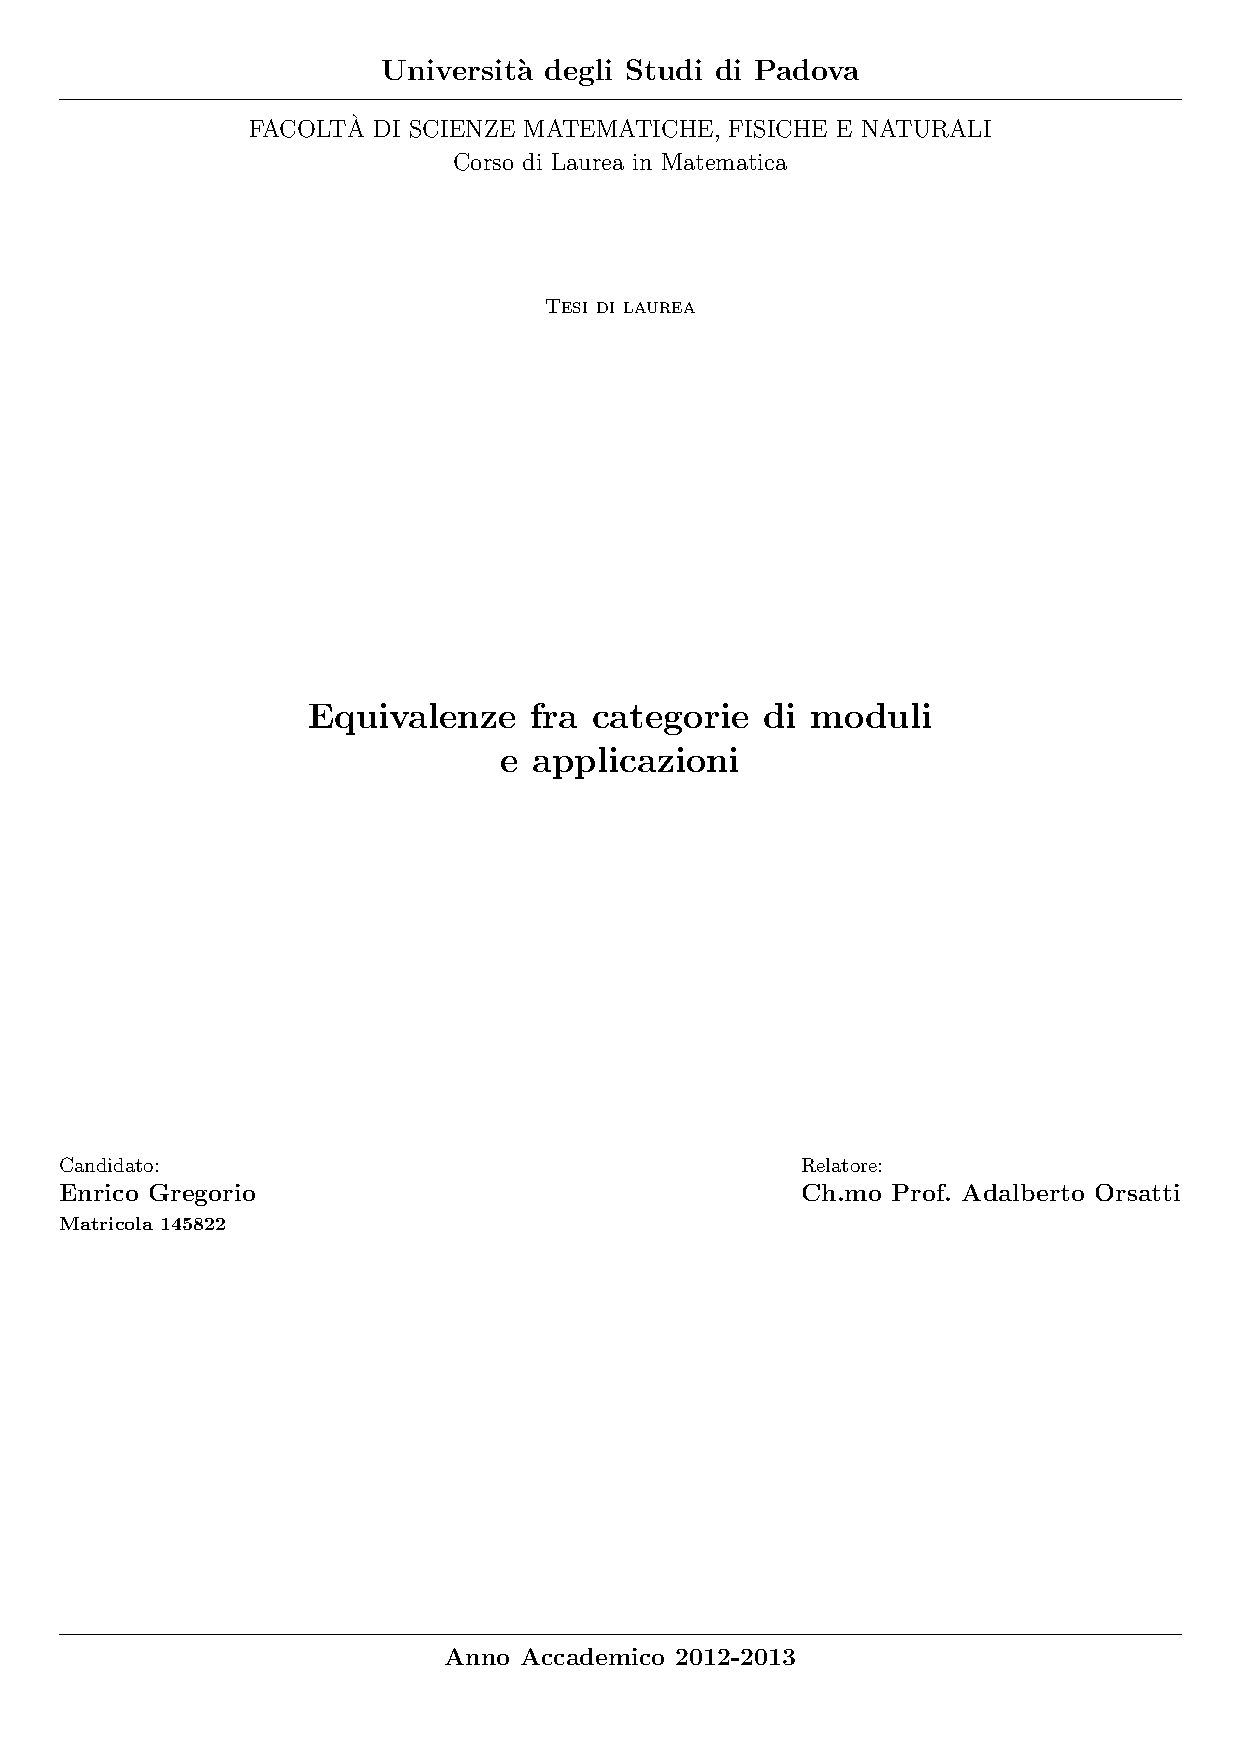
\includegraphics[width=0.95\linewidth]{images/frontespizio/frontespizio1-frn.pdf}}
    \subcaption{}\label{fig:frontespizio:A}
  \end{minipage}%
  \begin{minipage}[b]{.5\linewidth}
    \centering
    \fbox{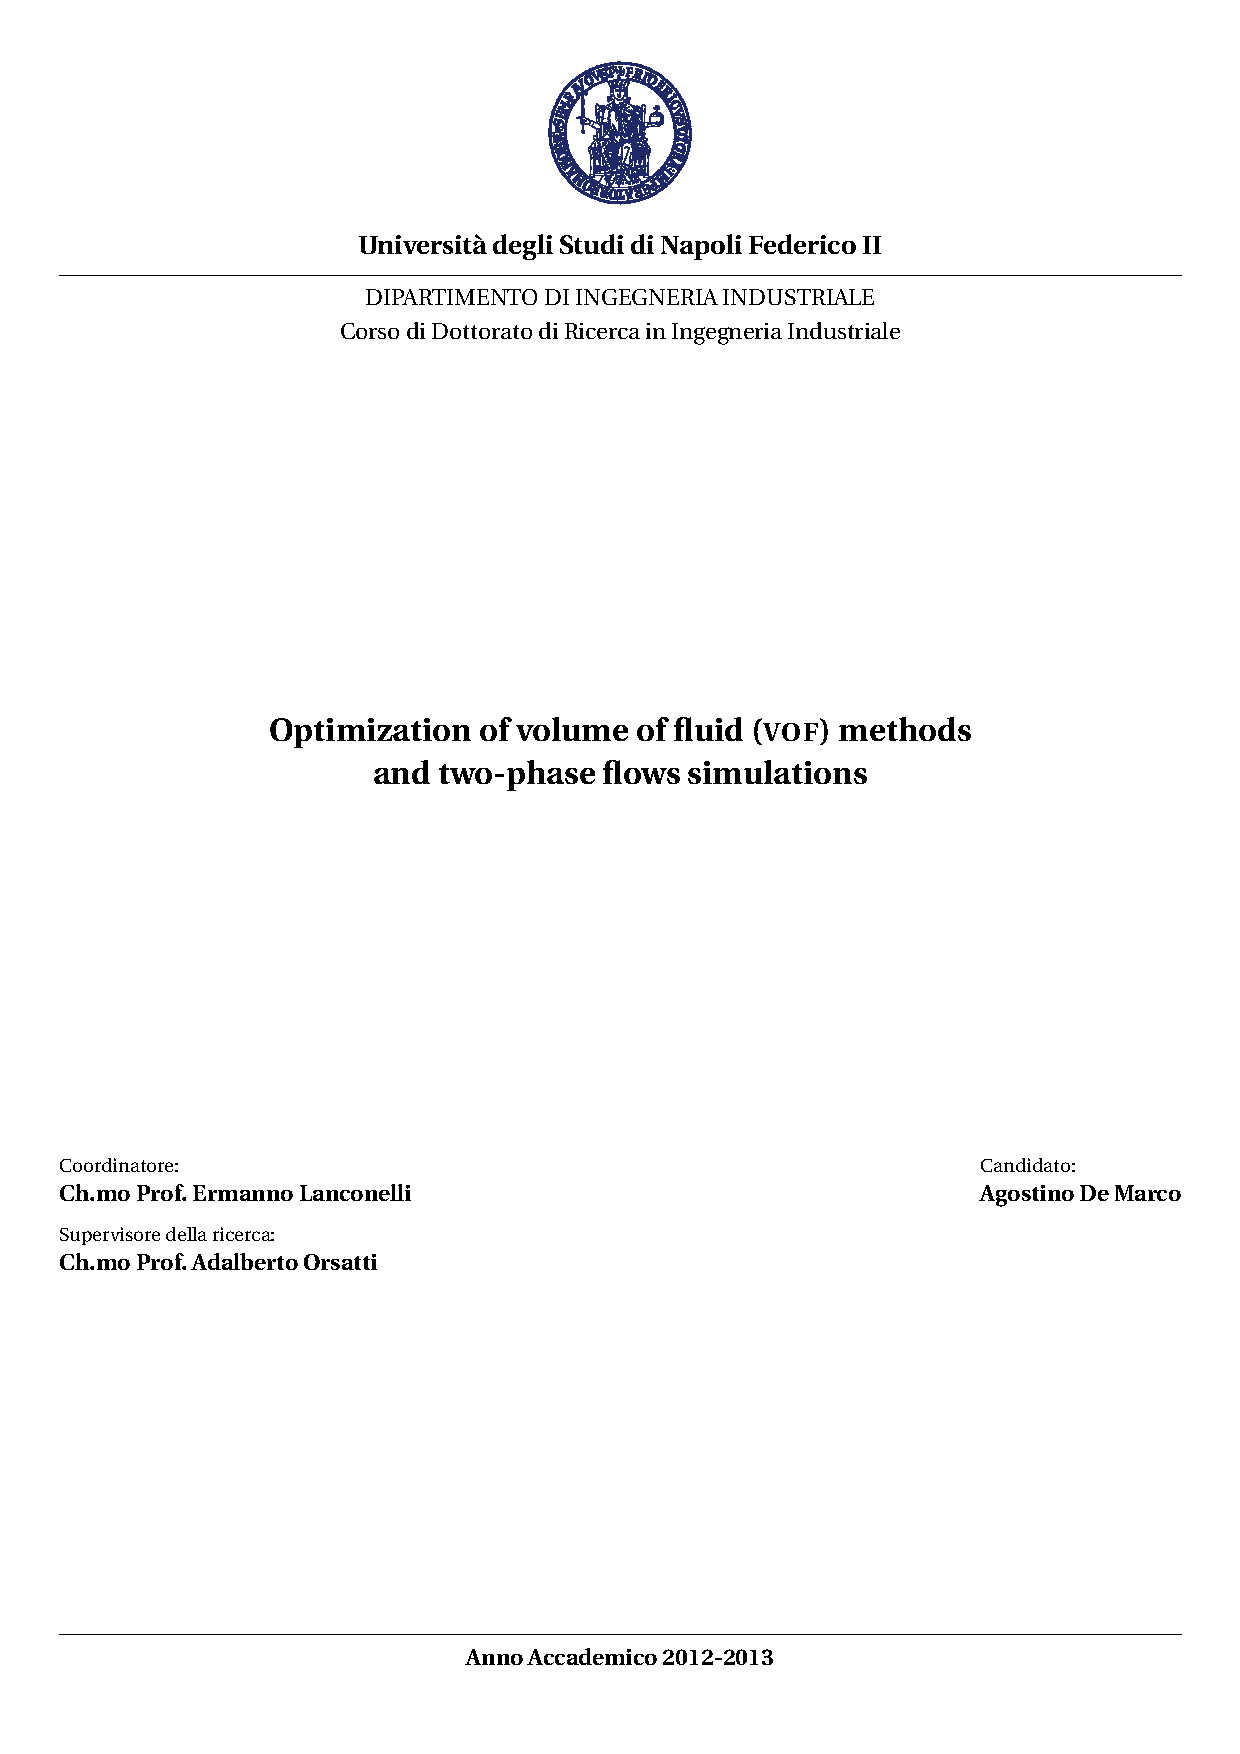
\includegraphics[width=0.95\linewidth]{images/frontespizio/frontespizio2-frn.pdf}}
    \subcaption{}\label{fig:frontespizio:B}
  \end{minipage}
  \caption{Esempi di frontespizio.}\label{fig:frontespizio}
\end{figure*}

L'organizzazione della tesi di laurea è argomento di specifici manuali di
scrittura \citep{eco,lesina,matric00,matric03} ed in particolar modo
della normativa ISO relativa alla presentazione dei rapporti
scientifici e tecnici \citet{man:UNI5966}. 
Molto dettagliata è la guida di \citet{Saper:Comunicare} liberamente scaricabile dal sito
del Politecnico di Torino. 
In questo paragrafo si propone una
possibile struttura per la tesi e si affrontano le problematiche
relative ad ogni sezione.

Una tesi può in generale presentarsi con la seguente
struttura:\footnote{Il simbolo * contraddistingue le sezioni
facoltative mentre $^\circ$
indica che le sezioni non devono essere presenti nell'indice.}\\[\baselineskip]

\begin{elencopar}{frontmatter}
    \item Il frontespizio$^\circ$%
    \item La dedica*$^\circ$%
    \item Il sommario*$^\circ$%
    \item I ringraziamenti*$^\circ$
    \item Gli indici$^\circ$%
    \item I simboli e le notazioni*%
    \item La prefazione*
\end{elencopar} \\[\spazz]
%
\begin{elencopar}{mainmatter}
    \item I capitoli interni
    \item Le appendici*%
\end{elencopar} \\[\spazz]
%
\begin{elencopar}{backmatter}
    \item La bibliografia%
    \item L'elenco degli acronimi*%
    \item L'indice analitico*%
\end{elencopar} \vspace{\baselineskip}

\section{Il frontespizio}
\label{sec:frontespizio}

La struttura ed il contenuto del frontespizio sono generalmente
imposti dalla scuola presso cui la laurea è conseguita, dunque è
necessario crearlo \emph{ad hoc}. 
Uno dei problemi che spesso si presentano è quello di
produrre un frontespizio adeguato che sia ben centrato sulla prima pagina.

Per gli utenti italiani esiste una soluzione già pronta e facilmente personalizzabile,
costituita dal pacchetto \ADMpacch{frontespizio}.
Il vantaggio di usare questo pacchetto è che i comandi necessari per definire i vari
elementi del frontespizio (titolo, candidato, relatore e così via) sono contenuti nello
stesso documento. 

Per definire il frontespizio si deve usare l'ambiente \verb+frontespizio+ che può essere
posizionato subito dopo il comando \verb+\begin{document}+. All'interno dell'ambiente
vanno dati i comandi che definiscono i vari elementi del frontespizio.
Se il documento principale si chiama \verb+tesi.tex+, alla prima compilazione verrà
generato automaticamente il documento \verb+tesi-frn.tex+, che si troverà nella stessa 
cartella che contiene quello principale. Il documento \verb+tesi-frn.tex+ va anch'esso 
compilato per generare il file \verb+tesi-frn.pdf+, che verrà posizionato automaticamente
come prima pagina di \verb+tesi.pdf+.
La sequenza di comandi è, dunque,

\smallskip
\noindent
\adjustbox{center=\linewidth,minipage=0.9\linewidth}{
  \verb+pdflatex tesi+\\
  \verb+pdflatex tesi-frn+\\
  \verb+pdflatex tesi+
}

\smallskip
\noindent
e, alla fine, il frontespizio sarà al suo posto.
Non occorrerà dare ogni volta questi comandi: basta farlo solo quando si modifica
il contenuto dell'ambiente \verb+frontespizio+.

Se la classe \class{book} è chiamata con l'opzione \verb+oneside+, 
il frontespizio occupa correttamente solo la prima pagina; nel caso di \verb+twoside+, 
viene prodotta una seconda pagina bianca.

Il documento va impostato dando al comando \texttt{\string\documentclass} l'opzione 
\verb+titlepage+ per poi caricare nel preambolo il pacchetto frontespizio. Per esempio:

\begin{tcblisting}{breakable,
  boxrule=0mm,arc=0mm,boxsep=-7pt,top=9pt,bottom=9pt,oversize,
  listing only,colback=gray!15,
  %listing options={}
}
\documentclass[a4paper,
  % ... altre opzioni
  titlepage]{book}
% ... altri comandi del preambolo
\usepackage{frontespizio}

\begin{document}
\begin{frontespizio}
\Universita{Padova}
\Facolta{Scienze Matematiche, Fisiche e Naturali}
\Corso[Laurea]{Matematica}
\Titoletto{Tesi di laurea}
\Titolo{Equivalenze fra categorie di moduli\\
e applicazioni}
\Candidato[145822]{Enrico Gregorio}
\Relatore{Ch.mo Prof.~Adalberto Orsatti}
\Annoaccademico{2012-2013}
\end{frontespizio}
% ... il resto della tesi
\end{document}
\end{tcblisting}

\noindent
produce il frontespizio riportato nella figura~\ref{fig:frontespizio:A}.
L'esempio seguente:

\begin{tcblisting}{breakable,
  boxrule=0mm,arc=0mm,boxsep=-7pt,top=9pt,bottom=9pt,oversize,
  listing only,colback=gray!15,
  %listing options={}
}
\documentclass[a4paper,titlepage]{book}
\usepackage[swapnames]{frontespizio}
\begin{document}
\begin{frontespizio}
\begin{Preambolo*}
\usepackage{fourier}
\newcommand{|\color{red!40!black}\verb+\VOF+|}{\textsc{vof}}
\end{Preambolo*}
\Universita{Napoli Federico II}
\Logo[2.5cm]{Sigillo_UNINA_FedericoII_BLUE}
\Dipartimento{Ingegneria Industriale}
\Corso[Dottorato di Ricerca]{Ingegneria Industriale}
\Titolo{Optimization of volume of fluid
  (|\color{red!40!black}\verb+\VOF+|) methods\\
  and two-phase flows simulations
}
\Candidato{Agostino~De~Marco}
\Relatore{Ch.mo Prof.~Ermanno Lanconelli}
\NRelatore{Coordinatore}{}
\Correlatore{Ch.mo Prof.~Adalberto Orsatti}
\NCorrelatore{Supervisore della ricerca}{}
\Annoaccademico{2012-2013}
\end{frontespizio}
...
\end{document}
\end{tcblisting}

\noindent
produce il frontespizio della figura~\ref{fig:frontespizio:B} e mostra
anche la possibilità di inserire un'immagine che rappresenta il logo dell'ateneo.

\section{La dedica}

La dedica, ove presente, può assumere le più svariate forme a seconda
dei gusti dell'autore. Di solito (vedi ad esempio la
figura~\ref{fig:dedica}) è costituita da una riga allineata a destra ad
esempio con i comandi
\begin{tcblisting}{breakable,
  boxrule=0mm,arc=0mm,boxsep=-7pt,top=9pt,bottom=9pt,oversize,
  listing only,colback=gray!15,
  %listing options={}
}
\begin{flushright}
...
\end{flushright}
\end{tcblisting}

La posizione verticale della riga nella pagina può essere scelta a
piacere e per controllarla risulta particolarmente conveniente l'uso
di una coppia di comandi \verb+\vspace{\stretch{...}}+. In questo
modo è infatti possibile impostare il rapporto tra lo spazio che
precede la dedica e quello che segue. Se ad esempio si vuole che lo
spazio che segue sia il doppio di quello che precede, è possibile
usare i comandi
\begin{tcblisting}{breakable,
  boxrule=0mm,arc=0mm,boxsep=-7pt,top=9pt,bottom=9pt,oversize,
  listing only,colback=gray!15,
  %listing options={}
}
\null\vspace{\stretch{1}}
\begin{flushright}
  \textit{A Valeria e ai miei genitori}
\end{flushright}
\vspace{\stretch{2}}\null
\end{tcblisting}

\begin{figure}[t]
\centering{%
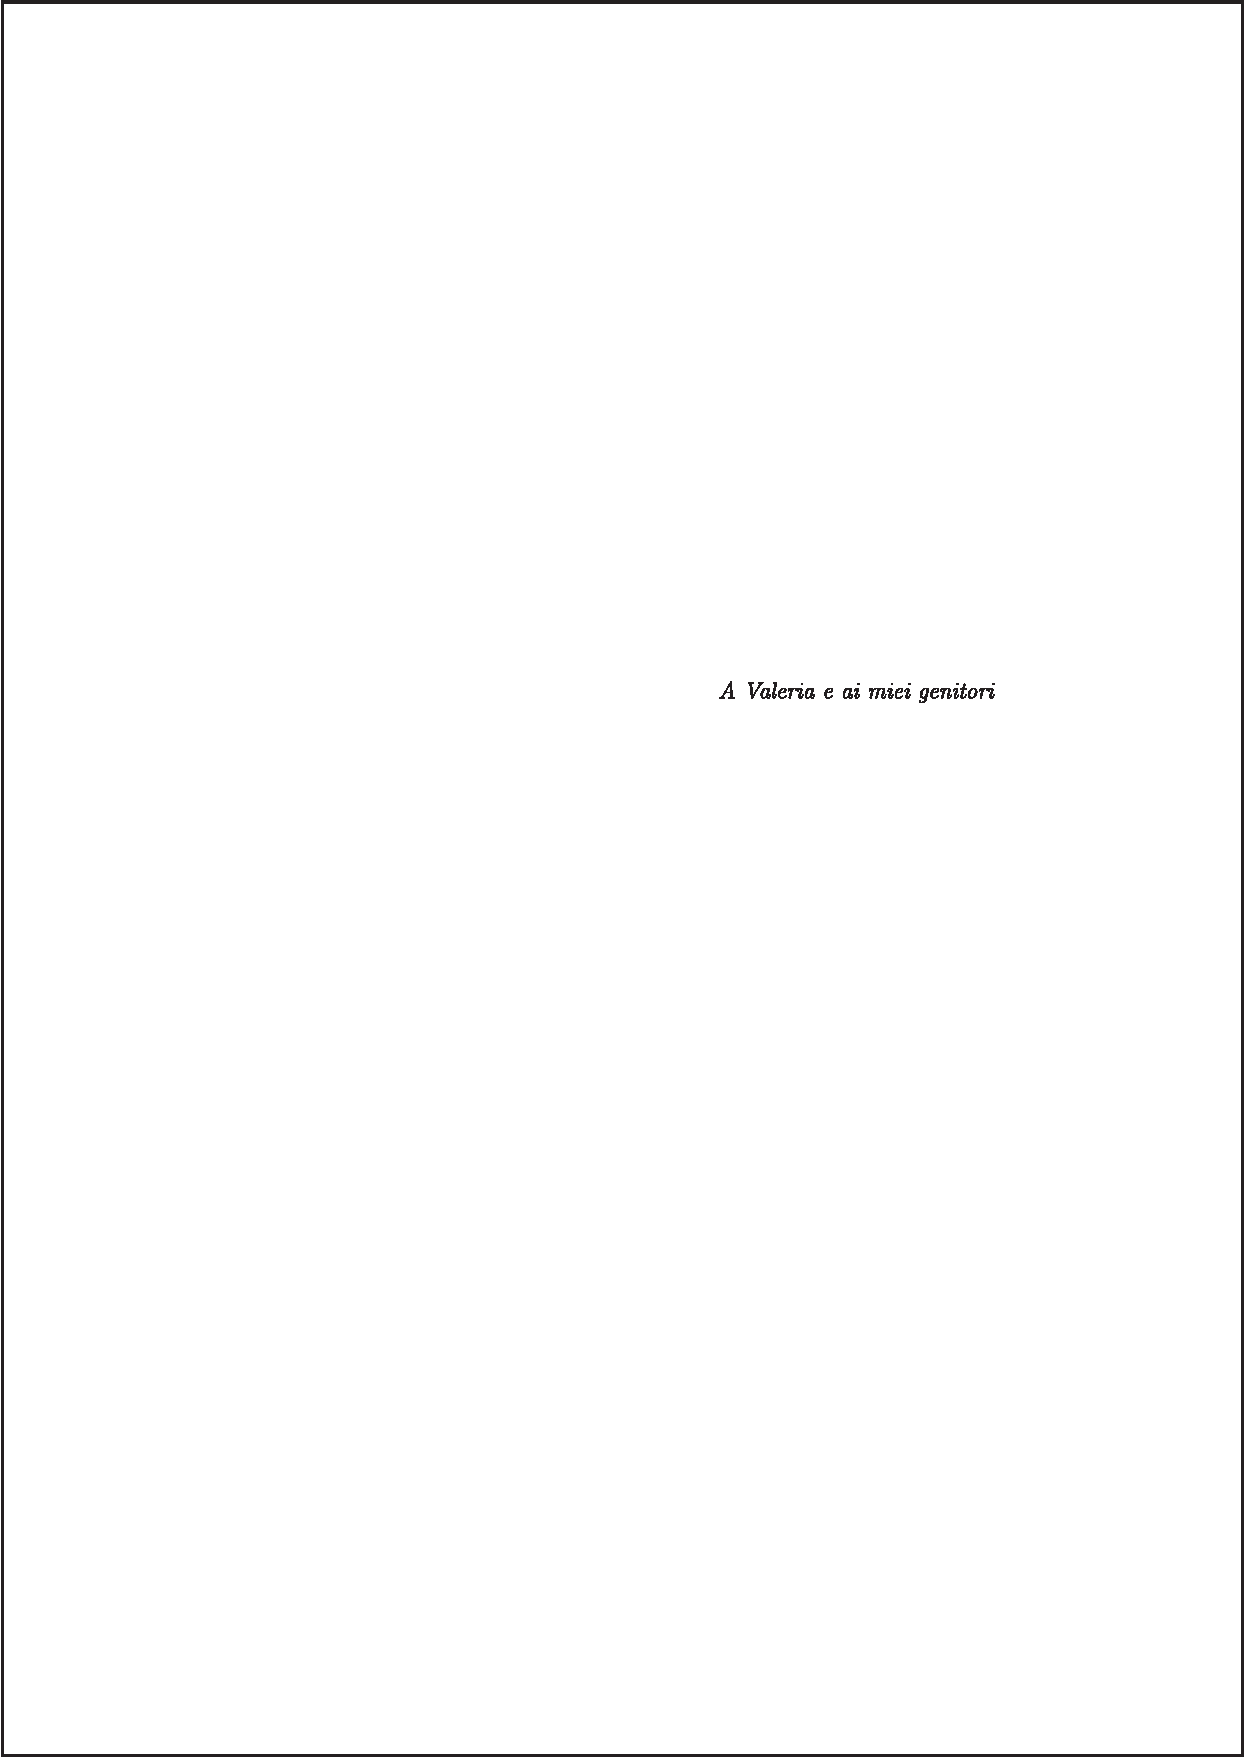
\includegraphics[width=\columnwidth]{images/dedica/dedica.pdf}}
\caption{Esempio di dedica.}\label{fig:dedica}
\end{figure}

\section{Il sommario}

Le classi \class{article} e \class{report} --- ma non di default la classe \class{book} ---
definiscono un ambiente
\begin{tcblisting}{breakable,
  boxrule=0mm,arc=0mm,boxsep=-7pt,top=9pt,bottom=9pt,oversize,
  listing only,colback=gray!15,
  %listing options={}
}
\begin{abstract}
...
\end{abstract}
\end{tcblisting}

\noindent
per il sommario o \emph{abstract} dei contenuti di un documento.
Se si utilizza la classe \class{book} è necessario inserire nel preambolo
la definizione di tale ambiente. Si riporta qui una definizione ispirata
a quella della classe \class{report}
\begin{tcblisting}{breakable,
  boxrule=0mm,arc=0mm,boxsep=-7pt,top=9pt,bottom=9pt,oversize,
  listing only,colback=gray!15,
  %listing options={}
}
|\color{green!40!black}\relsize{-1}\itshape nel preambolo|
\usepackage{fancyhdr}

\newenvironment{abstract}%
  {\cleardoublepage%
    \thispagestyle{empty}%
    \null \vfill\begin{center}%
      \bfseries \abstractname \end{center}}%
  {\vfill\null}
\end{tcblisting}
%
Si noti l'utilizzo del pacchetto \ADMpacch{fancyhdr} al quale si accennerà nel paragrafo~\ref{sec:testatine}.

Per le tesi di laurea in italiano è spesso richiesto che sia presente
anche la traduzione inglese dell'abstract. Utilizzando il pacchetto
\ADMpacch{babel} è possibile selezionare la lingua per le due versioni
dell'abstract in modo che sia effettuata la corretta sillabazione
delle parole e che sia caricato automaticamente il corretto titolo del
sommario. Dopo aver richiamato il pacchetto nel preambolo con il
comando
\begin{tcblisting}{breakable,
  boxrule=0mm,arc=0mm,boxsep=-7pt,top=9pt,bottom=9pt,oversize,
  listing only,colback=gray!15,
  %listing options={}
}
\usepackage[english,italian]{babel}
\end{tcblisting}

\noindent
è sufficiente inserire i sommari come segue

\begin{tcblisting}{breakable,
  boxrule=0mm,arc=0mm,boxsep=-7pt,top=9pt,bottom=9pt,oversize,
  listing only,colback=gray!15,
  %listing options={}
}
\begin{abstract}
... versione del sommario in italiano ...
\end{abstract}

\selectlanguage{english}
\begin{abstract}
... English version of the abstract ...
\end{abstract}
\selectlanguage{italian}
\end{tcblisting}

Il risultato è riportato nella figura~\ref{fig:abstract}.

\begin{figure*}[tb]
  \begin{minipage}[b]{.5\linewidth}
    \centering
    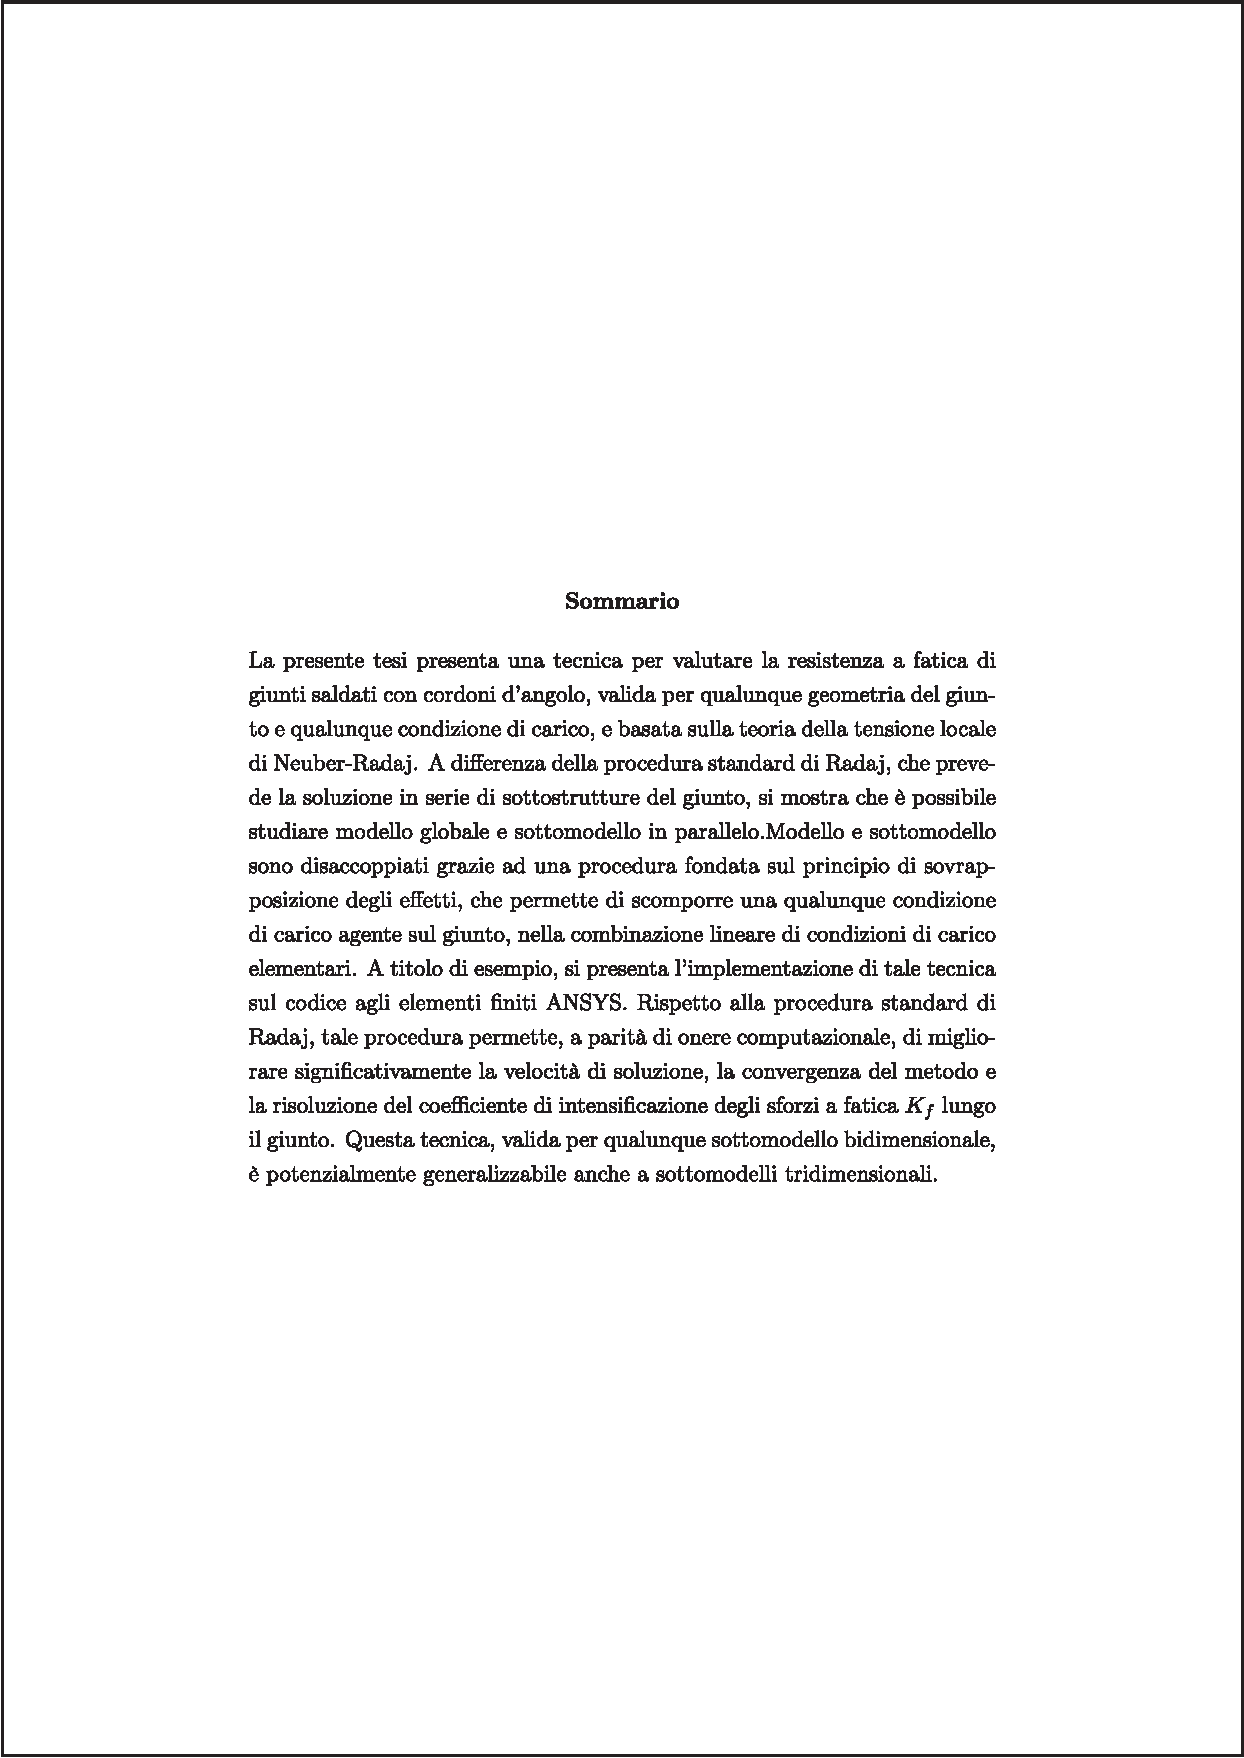
\includegraphics[width=0.95\linewidth]{images/abstract/abstract1.pdf}
    \subcaption{}\label{fig:abstract:A}
  \end{minipage}%
  \begin{minipage}[b]{.5\linewidth}
    \centering
    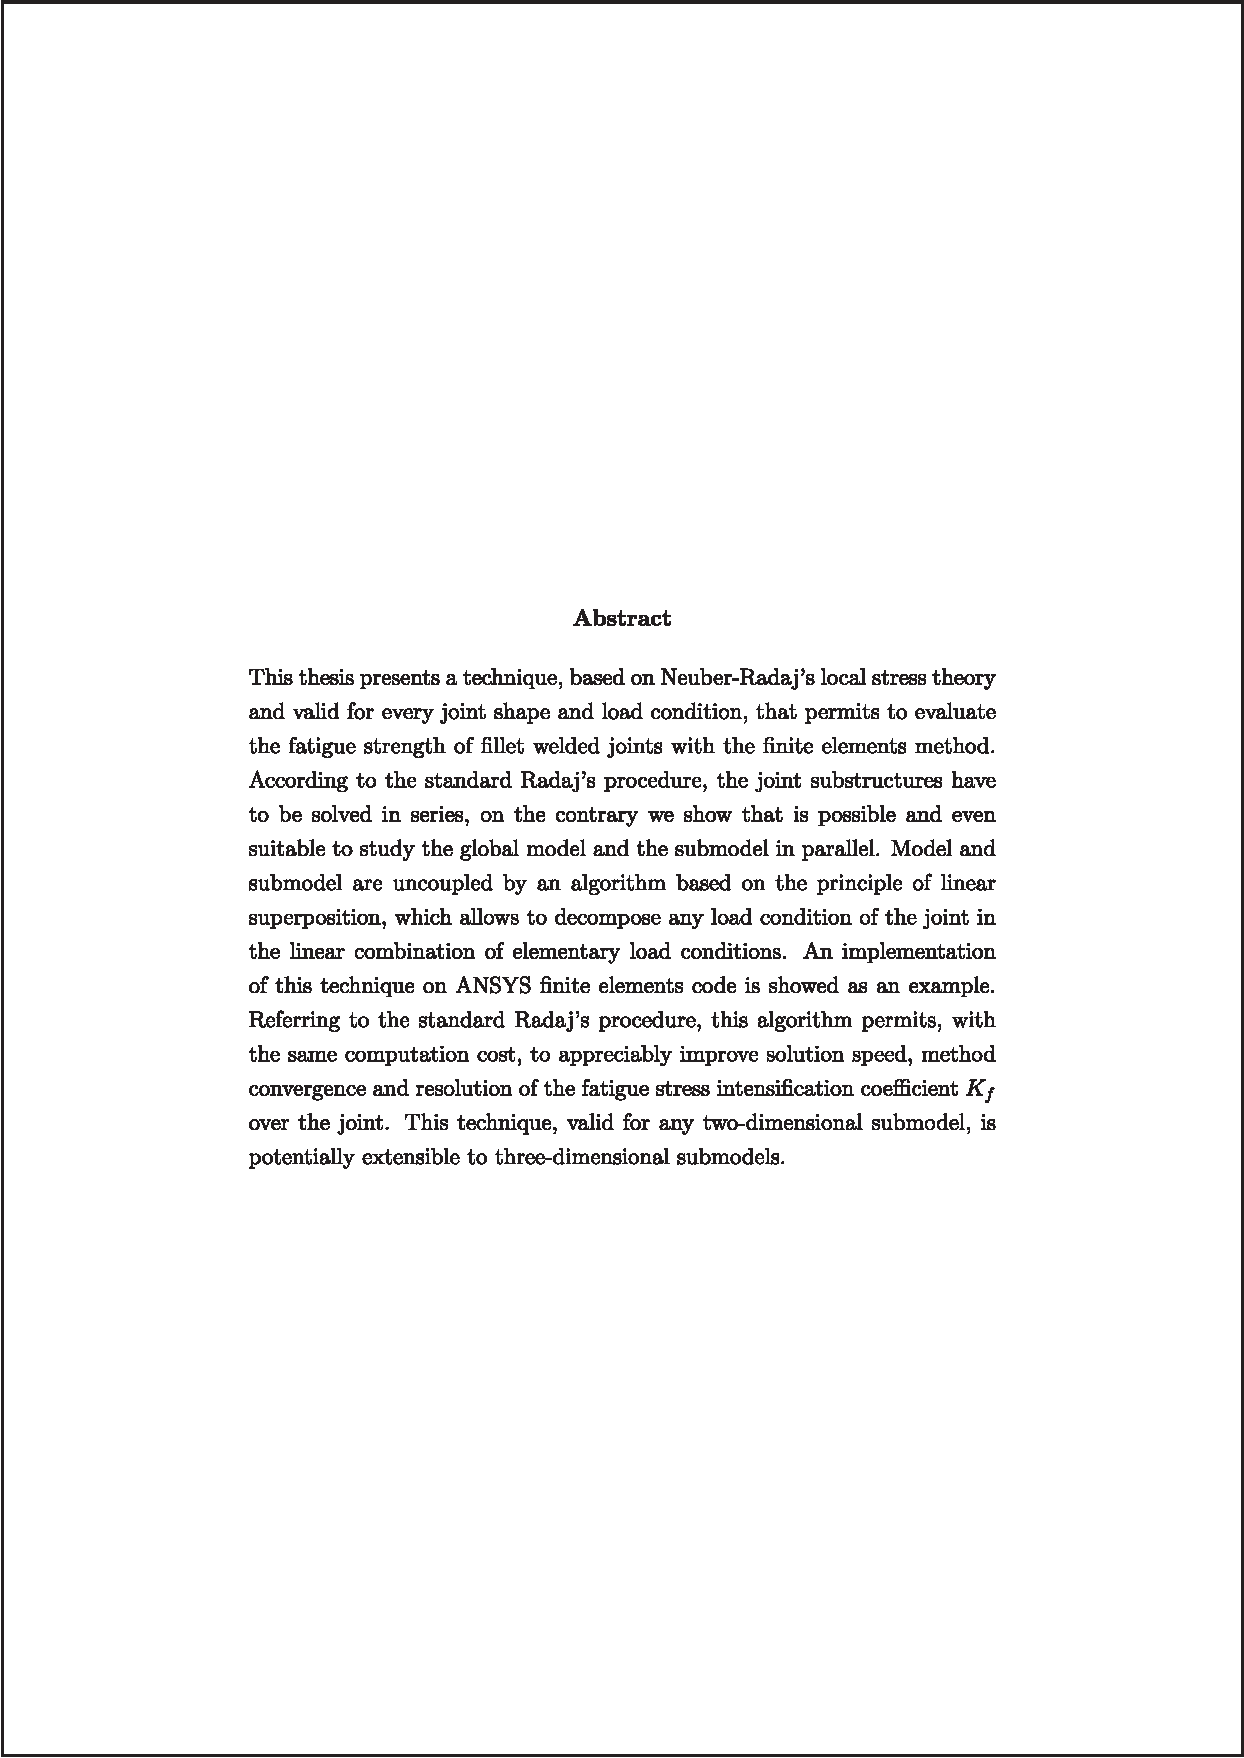
\includegraphics[width=0.95\linewidth]{images/abstract/abstract2.pdf}
    \subcaption{}\label{fig:abstract:B}
  \end{minipage}
  \caption{Esempio di abstract in doppia lingua.}\label{fig:abstract}
\end{figure*}

\section{Gli indici}

Gli indici di solito sono posizionati subito dopo il sommario nel
seguente ordine:
\begin{compactitemize}
    \item indice
    \item elenco delle figure
    \item elenco delle tabelle
    \item altri elenchi
\end{compactitemize}
e vengono prodotti automaticamente da \LaTeX{} con i comandi
\begin{tcblisting}{breakable,
  boxrule=0mm,arc=0mm,boxsep=-7pt,top=9pt,bottom=9pt,oversize,
  listing only,colback=gray!15,
  %listing options={}
}
\tableofcontents
\listoffigures
\listoftables
\end{tcblisting}

Per creare elenchi di oggetti flottanti personalizzati (ad esempio
listati di programmi, algoritmi, eccetera) si faccia riferimento al
pacchetto \ADMpacch{float} ed ai relativi comandi \verb+\newfloat+ e
\verb+\listof+. Per modificare il layout degli indici è possibile
utilizzare il pacchetto \ADMpacch{tocloft}.

\section{I simboli e le notazioni}

Talvolta risulta opportuno far precedere al testo della tesi un
elenco dei simboli e delle notazioni utilizzate. A questo scopo può
essere utilizzato il pacchetto \ADMpacch{nomencl}.
Un'alternativa più potente a \ADMpacch{nomencl} è il pacchetto \ADMpacch{glossaries}
che permette anche di creare un elenco degli acronimi menzionati nel testo e un glossario.
Entrambi i pacchetti generano gli elenchi automaticamente per mezzo del programma \texttt{makeindex}
e, accoppiati all'uso del pacchetto \ADMpacch{hyperref},
generano automaticamente anche i collegamenti ipertestuali tra il simbolo, l'acronimo, 
il termine menzionato nel testo e la relativa spiegazione nell'elenco.
Si rimanda ai rispettivi manuali d'uso per approfondimenti.

Ovviamente, per semplicità, è anche possibile creare manualmente l'elenco, ad esempio
utilizzando l'ambiente \amb{tabular}. Nella figura~\ref{fig:simboli} si
riporta un esempio.

\begin{figure*}[tb]
\centering{%
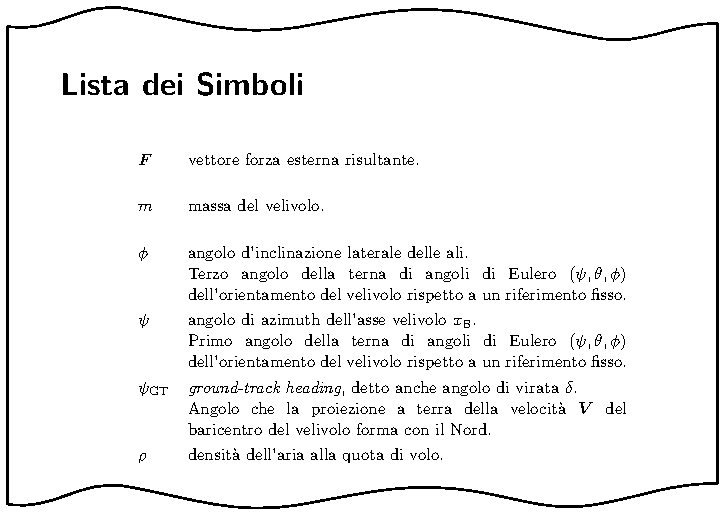
\includegraphics[width=0.8\textwidth]{images/simboli/symbols.pdf}}
\caption{Esempio di elenco dei simboli.}\label{fig:simboli}
\end{figure*}

\section{Le appendici}

Le appendici sono dei normali capitoli la cui numerazione è però in
lettere latine. \LaTeX{} permette di crearle semplicemente con il
comando \verb+\chapter{...}+ preceduto da \verb+\appendix+; se si
hanno più appendici, \verb+\appendix+ deve essere richiamato solo una
volta. Si riporta un esempio:
\begin{tcblisting}{breakable,
  boxrule=0mm,arc=0mm,boxsep=-7pt,top=9pt,bottom=9pt,oversize,
  listing only,colback=gray!15,
  %listing options={}
}
...
\mainmatter
\include{capitolo1}
\include{capitolo2}
\include{capitolo3}

\appendix
\include{appendice1}
\include{appendice2}
...
\end{tcblisting}

\section{L'indice analitico}

L'indice analitico può essere creato automaticamente per mezzo del
pacchetto \pack{imakeidx}. 

L'esempio seguente:
\begin{tcblisting}{breakable,
  boxrule=0mm,arc=0mm,boxsep=-7pt,top=9pt,bottom=9pt,oversize,
  listing only,colback=gray!15,
  %listing options={}
}
\usepackage{imakeidx}
...
\makeindex[title=Concept index]
\makeindex[name=persons,title=Index of names,columns=3]
...
\begin{document}
...
la relatività.\index{relativity}
...
Einstein.\index[persone]{Einstein, Albert}
...
E fu da quel punto che fu data alla teoria il 
nome di \emph{Teoria della relatività}.

\printindex

\indexprologue{\small 
  In questo indice troverete un elenco 
  di scienziati famosi citati in questa
  tesi.
}
\printindex[persone]

\end{document}
\end{tcblisting}

\noindent
produce due indici analitici. Il secondo è preceduto da un breve testo
di spiegazione.

Si rimanda al manuale d'uso del pacchetto per le eventuali necessità
di personalizzazione del formato.

\section{La bibliografia}

La bibliografia è una parte importante della tesi di laurea.
\LaTeX{} offre tutti gli strumenti per realizzarla
e gestirla con efficienza e flessibilità. L'argomento richiede la comprensione
di alcuni aspetti tecnici e, al solito, si consiglia di approfondirne
i dettagli consultando la guida di \citeauthor{man:Pantieri}.
Qui si richiamano gli elementi fondamentali per gestire le citazioni bibliografiche
e il database delle fonti con il pacchetto \ADMpacch{biblatex}.

La gestione efficiente della bibliografia è basata sulla generazione automatica
di un insieme di voci bibliografiche citate durante il testo della tesi.
Le voci bibliografiche vengono `estratte'
da una collezione (database) di fonti preparata in precedenza.
Il database è un file di testo di estensione \verb+.bib+ che va editato a parte
inserendovi dei record opportunamente formattati.
Esiste un ottimo programma multipiattaforma per la creazione di database 
bibliografici chiamato Jabref.\footnote{\url{http://jabref.sourceforge.net}}
Esso è dotato di un'interfaccia grafica e di potenti funzioni di gestione.

Un esempio di database bibliografico contenente un certo numero di record è il seguente:
\begin{tcblisting}{breakable,
  boxrule=0mm,arc=0mm,boxsep=-7pt,top=9pt,bottom=9pt,oversize,
  listing only,colback=gray!15,
  %listing options={}
}
|\color{red!70!black}\ttfamily\bfseries @book|{|\color{blue!70!black}eco:tesi|,
  author = {Eco, Umberto},
  title = {Come si fa una tesi di laurea},
  publisher = {Bompiani},
  date = {1977},
  location = {Milano},
}

|\color{red!70!black}\ttfamily\bfseries @article|{|\color{blue!70!black}mori:tesi|,
  author = {Mori, Lapo Filippo},
  title = {Scrivere la tesi di laurea con \LaTeX},
  journaltitle = {\Ars},
  number = {3},
  date = {2007},
}

|\color{red!70!black}\ttfamily\bfseries @manual|{|\color{blue!70!black}beccari:gordini:codifiche|,
  title = {Codifiche in {\TeX} e {\LaTeX}. Dal sorgente al PDF, guida pratica per lavorare con successo.},
  author = {Beccari, Claudio and Gordini, Tommaso},
  publisher = {{\GuIT}},
  year = {2012},
}

|\color{red!70!black}\ttfamily\bfseries @online|{|\color{blue!70!black}wiki:latex|,
  title = {\LaTeX{} su Wikipedia},
  date = {2012},
  url = {http://it.wikipedia.org/wiki/LaTeX},
  sortkey = {wiki},
  label = {wiki},
}
\end{tcblisting}

\noindent
Il primo record è un esempio di voce bibliografica riferita a un libro (\verb+@book+),
il secondo è un esempio di articolo su rivista (\verb+@article+).
il terzo record è un riferimento a un manuale (\verb+@manual+), 
il quarto è un sito internet (\verb+@online+).

Ciascun record ha dei campi che vanno dal titolo, all'autore, all'anno di pubblicazione,
e così via.%
\footnote{%
  ciascun campo, come si vede, va terminato con la virgola, \emph{anche se è l'ultimo}, 
  pena un errore.
}
I record sono identificati da una \emph{chiave}; per esempio il record del
libro di Eco ha per chiave \verb+eco:tesi+. Le chiavi vengono stabilite dall'utente
e devono essere usate nel testo della tesi allorquando si vuole inserire una citazione 
bibliografica.

Il programma `estrattore' delle voci bibliografiche dal file \verb+.bib+,
che lavora tenendo conto delle effettive citazioni presenti nella tesi,
si chiama \texttt{biber} e fa parte delle moderne distribuzioni \TeX{}.
%Il programma \texttt{biber} produce anche una determinata formattazione 
%della bibliografia --- \emph{stile} di citazione bibliografica ---
%attraverso appositi file di stile (di estensione \verb+.bst+).

Il pacchetto \ADMpacch{biblatex} è un potentissimo strumento --- pensato per
interfacciarsi con \verb+biber+ --- con il quale si gestisce 
automaticamente la bibliografia e si personalizza ogni aspetto degli stili 
bibliografici e di citazione con poche operazioni.
Per funzionare correttamente, il pacchetto richiede di caricare anche il pacchetto 
\ADMpacch{babel} (o \ADMpacch{polyglossia}, se si compone con \XeLaTeX) e 
\ADMpacch{csquotes} con le opzioni indicate di seguito.

Nel preambolo vanno dati i comandi:
\begin{tcblisting}{breakable,
  boxrule=0mm,arc=0mm,boxsep=-7pt,top=9pt,bottom=9pt,oversize,
  listing only,colback=gray!15,
  %listing options={}
}
\usepackage[italian]{babel}% tesi in italiano

\usepackage[
    autostyle,italian=guillemets
    % ... altre opzioni
  ]{csquotes}

\usepackage[
    % ... opzioni
    backend=biber
  ]{biblatex}
\end{tcblisting}


Se, per esempio, la base di dati è stata nominata \verb+bibliografia-tesi.bib+,
per indicare a \LaTeX{} di usare questo file per comporre la bibliografia,
si deve dare nel preambolo il comando
\begin{tcblisting}{breakable,
  boxrule=0mm,arc=0mm,boxsep=-7pt,top=9pt,bottom=9pt,oversize,
  listing only,colback=gray!15,
  %listing options={}
}
\addbibresource{bibliografia-tesi.bib}
\end{tcblisting}
Se si ha più di un database bibliografico, il comando precedente deve essere
ripetuto per ogni file e specificando sempre l'estensione \verb+.bib+.

A questo punto, nel testo della tesi, la citazione di una fonte bibliografica sarà 
semplicemente ottenuta con un qualcosa di simile:
\begin{tcblisting}{breakable,
  boxrule=0mm,arc=0mm,boxsep=-7pt,top=9pt,bottom=9pt,oversize,
  listing only,colback=gray!15,
  %listing options={}
}
Si veda~\cite{eco:tesi} per maggiori dettagli.
\end{tcblisting}

\noindent
cioè con il comando \verb+\cite+.
Per ottenere il risultato voluto, che potrebbe essere il seguente:%
\begin{quote}
Si veda~[1] per maggiori dettagli.
\end{quote}
la sequenza di comandi di compilazione è:

\medskip
\noindent
\adjustbox{center=\linewidth,minipage=0.9\linewidth}{
  \verb+pdflatex tesi+\\
  \verb+biber tesi+\\
  \verb+pdflatex tesi+\\
  \verb+pdflatex tesi+
}

\medskip
\noindent
Ovviamente questa sequenza è richiesta solo quando si modifica
%il database 
\verb+bibliografia-tesi.bib+ (per esempio, dopo aver aggiunto una voce o
aver corretto un errore).
La doppia compilazione con \verb+pdflatex+ dopo l'esecuzione di \verb+biber+
è necessaria per la corretta gestione delle informazioni trascritte nei file ausiliari.

Si osservi che il formato finale della citazione dipende dallo stile 
richiesto tramite le opzioni passate al pacchetto \ADMpacch{biblatex}.
L'esempio precedente potrebbe avere l'aspetto seguente:
\begin{quote}
Si veda~\textsc{eco}~(1977) per maggiori dettagli.
\end{quote}
in cui lo stile della citazione è passato da quello `numerico' a quello
cosiddetto `autore-anno'.

Il comando \verb+\printbibliography+ posizionato
al termine del testo della tesi produce la \emph{sezione bibliografica} con relativi
titolo e testatina. La sezione bibliografica non è altro che l'elenco dei riferimenti
bibliografici, opportunamente ordinati e formattati.

Per mandare nell'indice generale il titolo della bibliografia del documento,
va data la sequenza di comandi seguente (valida per la classe di documento \verb+book+):
\begin{tcblisting}{breakable,
  boxrule=0mm,arc=0mm,boxsep=-7pt,top=9pt,bottom=9pt,oversize,
  listing only,colback=gray!15,
  %listing options={}
}
\addcontentsline{toc}{|chapter|}{\bibname}
\printbibliography
\end{tcblisting}

Se si usa \verb+babel+ per un documento in italiano il 
comando \verb+\bibname+ produce nell'indice generale del documento la
voce \emph{Bibliografia}. Se nell'indice si vuole la voce 
\emph{Riferimenti bibliografici} basta ridefinire \verb+\bibname+
tramite il comando
\begin{tcblisting}{breakable,
  boxrule=0mm,arc=0mm,boxsep=-7pt,top=9pt,bottom=9pt,oversize,
  listing only,colback=gray!15,
  %listing options={}
}
\addto\captionsitalian{%
  \renewcommand*{\bibname}%
    {Riferimenti bibliografici}%
}
\end{tcblisting}

Si osservi che l'aspetto dei riferimenti bibliografici e delle citazioni, 
che \ADMpacch{biblatex} adatta automaticamente alla lingua principale del documento, 
si specificano in diversi modi.
Il pacchetto fornisce quattro stili bibliografici predefiniti, i quali
agiscono nella sezione bibliografica del documento.
Essi ordinano le opere (ad esempio, alfabeticamente in base al cognome di autore o
curatore); possono contrassegnare o meno l'opera con un'etichetta;
sistemano opportunamente i dati nei riferimenti bibliografici.

Si rimanda all'\emph{Arte} di \citeauthor{man:Pantieri} o al manuale
di \ADMpacch{biblatex} \citep{Lehman:biblatex} per approfondimenti sugli stili e sugli schemi di 
citazione.

\chapter{Gli oggetti}

\section{Le figure}

Le figure sono uno degli argomenti trattati più estesamente dalle
guide.
Al solito, l'\emph{Arte} di \citeauthor{man:Pantieri} è un'ottima fonte
di approfondimento.

I problemi incontrati dagli utenti \LaTeX{} durante l'inserimento di figure 
sono generalmente di due tipi. Una parte dei problemi derivano dalle figure 
in sé, ovvero dal file che si cerca di inserire in un documento
(verrà trattato nel par.~\ref{sec:formati}), 
mentre un altro tipo di problemi, totalmente
distinto dal precedente, è quello degli oggetti flottanti
(e verrà trattato nel par.~\ref{sec:flottanti}).

\subsection{Formati}
\label{sec:formati}

Esistono due grandi classi di figure, le immagini vettoriali e le
immagini bitmap. Le prime sono descritte da forme e possono essere
scalate e/o deformate senza perdere definizione; sono soprattutto
adatte per i grafici e per gli schemi. Le seconde sono matrici di
pixel colorati e sono adatte per le fotografie.

La prima cosa da fare è produrre figure nel formato più adatto per i
propri scopi. \`{E} inutile salvare grafici o schemi in
\texttt{.jpeg} per poi convertirli in \texttt{.pdf}, in quanto la
conversione di un'immagine bitmap in \texttt{.pdf} include
semplicemente il file bitmap in una ``cornice'' (tipica del formato
Encapsulated PostScript, da cui il PDF deriva) senza
migliorare in alcun modo la qualità. \`{E} inutile anche fare la
conversione opposta, da file vettoriale a bitmap, perché in questo
modo si perdono le informazioni sulla geometria contenuta nella
figura e quindi si abbassa la qualità del file.

L'elemento più importante di un file PDF è il Bounding Box
(BB), che determina la taglia effettiva dell'immagine e che serve
a \LaTeX{} per calcolare lo spazio da riservare alla figura.
Idealmente i BB dovrebbero essere al limite massimo del contenuto
dell'immagine, ma spesso i programmi di grafica lasciano grandi bordi
bianchi attorno alla figura disegnata. Questo porta spesso a grandi
confusioni, perché di fatto \LaTeX{} sta lasciando alla figura lo
spazio corretto, ma visivamente parte di questo è utilizzato per il
bordo bianco, quindi la figura appare troppo piccola, non centrata,
con eccessivi margini verticali, eccetera. La prima cosa da verificare è
quindi che il programma di grafica generi dei file \texttt{.pdf}
con BB corretti. Per farlo basta aprire la figura con 
Ghostview\footnote{\url{http://pages.cs.wisc.edu/~ghost}} e
attivare la visualizzazione dei BB. Se questi non sono corretti
bisogna cercare di configurare correttamente il programma di grafica,
ma il problema non ha niente a che vedere con \LaTeX{}. 
Nel caso si
abbiano molti file che presentano questo inconveniente bisogna cercare
di correggere il problema all'origine.

\subsection{Pacchetti utili}
\label{unix}

Per inserire le figure è necessario caricare il pacchetto
\ADMpacch{graphicx}, della cui guida si consiglia la lettura. Per
ottenere sottofigure (vedi ad esempio la figura.~\ref{fig:frontespizio}) è
necessario caricare il pacchetto \ADMpacch{subcaption}.

In casi semplici non è necessario ricorrere a quest'ultimo pacchetto
visto che all'interno degli ambienti \amb{figure} e \amb{table}
si può mettere più di un grafico o di una tabella. Se si hanno quindi
due o più figure che possono essere raggruppate insieme, scrivendo

\begin{tcblisting}{breakable,
  boxrule=0mm,arc=0mm,boxsep=-7pt,top=9pt,bottom=9pt,oversize,
  listing only,colback=gray!15,
  %listing options={}
}
\begin{figure}[tb]
  \begin{minipage}{0.48\textwidth}
    \includegraphics[%
      width=\linewidth]{fig_a.pdf}
    \caption{Prima didascalia (destra).}
    \label{fig:a}
  \end{minipage}
  \hspace{4em}
  \begin{minipage}{0.48\textwidth}
    \includegraphics[%
      width=\linewidth]{fig_b.pdf}
    \caption{Seconda didascalia (sinistra).}
    \label{fig:b}
  \end{minipage}
\end{figure}
\end{tcblisting}

In questo modo si riduce il numero di oggetti flottanti e se ne
facilita l'inserimento.

Al fine di mantenere ordine nei file sorgenti, è consigliabile
raccogliere tutte le figure in una o più sottocartelle; se ad esempio
tali sottocartelle si chiamano \verb+dir_1+ e \verb+dir_2+, è
sufficiente inserire nel preambolo con il seguente comando del pacchetto
\ADMpacch{graphicx}:
\begin{tcblisting}{breakable,
  boxrule=0mm,arc=0mm,boxsep=-7pt,top=9pt,bottom=9pt,oversize,
  listing only,colback=gray!15,
  %listing options={}
}
\graphicspath{{dir_1/},{dir_2/}}
\end{tcblisting}

L'argomento di \verb+\graphicspath+ è relativo alla cartella
dove risiede il main file \verb+.tex+ che viene compilato.

La formattazione delle didascalie può essere convenientemente
controllata con il pacchetto \ADMpacch{caption}.

Qui vale la pena di menzionare il pacchetto di estensione \ADMpacch{adjustbox}
che, tra le sue svariate funzionalità, offre il comando
\verb+\adjincludegraphics+ (simile a \verb+\includegraphics+)
che permette di effettuare agevoli operazioni di rifilatura (\emph{cropping}).
Ad esempio il codice
\begin{tcblisting}{breakable,
  boxrule=0mm,arc=0mm,boxsep=-7pt,top=9pt,bottom=9pt,oversize,
  listing only,colback=gray!15,
  %listing options={}
}
\adjincludegraphics[width=0.7\linewidth,
  trim={{.05\width} {.02\height} 0 0},% lbrt
  clip]{mia-figura.pdf}
\end{tcblisting}

\noindent
inserisce l'immagine \verb+mia-figura.pdf+
ritagliandone dal lato sinistro (\verb+l+, \emph{left}) una striscia 
di larghezza pari al 5\% della larghezza originale e dal lato in basso (\verb+b+, \emph{bottom})
una striscia di altezza uguale a 2\% dell'altezza originale. Il risultato
del ritaglio viene poi scalato in modo da avere un'immagine
sulla pagina di larghezza uguale al 70\% della \verb+\linewidth+.

\section{Le tabelle}

Così come per le figure, anche per le tabelle esistono guide
specifiche a cui si rimanda per ogni approfondimento
\cite{mori:arstexnica06}.

Per migliorare la spaziatura dell'ambiente \ADMpacch{tabular} standard è
possibile utilizzare il pacchetto \ADMpacch{ctable}, mentre se si
vogliono colorare le righe o le colonne è necessario caricare il
pacchetto \ADMpacch{xcolor} con l'opzione \verb+table+. 

Nel caso di tabelle di grandi dimensioni è possibile
ridurre la dimensione della tabella effettuando una
scalatura, ad esempio con i seguenti comandi:
\begin{tcblisting}{breakable,
  boxrule=0mm,arc=0mm,boxsep=-7pt,top=9pt,bottom=9pt,oversize,
  listing only,colback=gray!15,
  %listing options={}
}
\begin{center}
  \resizebox{0.95\textwidth}{!}{%
    \begin{tabular}
      ...
    \end{tabular}
  }
\end{center}
\end{tcblisting}

Si può anche ruotare la tabella di $90^\circ$ con il pacchetto
\ADMpacch{rotating}.
Altre tecniche per ruotare immagini e tabelle 
sono indicate nel manuale del pacchetto \ADMpacch{hvfloat} \citep{voss:hvfloat}.

Infine, si può spezzare la tabella su più pagine con il versatile pacchetto
\ADMpacch{longtable}.

\section{Controllo degli oggetti flottanti}
\label{sec:flottanti}

Spesso gli utenti si lamentano del fatto che \LaTeX\ sposti le
figure (e in generale gli oggetti flottanti) lontano dal punto in cui
vengono inserite. Nella maggioranza dei casi questo è dovuto ad un
utilizzo erroneo delle opzioni di posizionamento degli oggetti
flottanti. Qui si vuole sottolineare che alcune scelte
devono essere prese nella fase di stesura del testo
(paragrafo~\ref{sec:stesura}) mentre altre sono riservate, quando necessarie,
alla fase di revisione (paragrafo~\ref{revisione}).

\subsection{Cosa fare durante la stesura del testo}
\label{sec:stesura}

In primo luogo bisogna accettare il fatto che se \LaTeX\ sposta un
oggetto flottante è perché lo spazio è fisicamente insufficiente, o
per motivi estetico-tipografici. Per esempio \LaTeX\ non metterà mai
una figura seguita da un titolo di sezione e da un cambio pagina, ma
preferirà stampare la sezione e poi la figura, oppure se si aggiunge
un oggetto flottante in fondo ad una pagina, \LaTeX\ è obbligato a
spostarlo almeno nella pagina successiva. Se lo spazio è
insufficiente, è inutile cercare di forzare \LaTeX\ a mettere
l'oggetto flottante in tale posizione: se lo spazio fisico non c'è,
non si può certo inventarlo.

Per fortuna con un minimo di accortezza \LaTeX\ fa un ottimo lavoro.
Per prima cosa è opportuno utilizzare sempre il posizionamento
automatico evitando di aggiungere \verb+\clearpage+ o comandi simili:
in fase di redazione chi scrive la tesi dovrebbe solo concentrarsi sui 
contenuti e non sull'impaginazione. In generale i posizionamenti fatti a mano
interferiscono con la complessa routine di \LaTeX\ per il
posizionamento degli oggetti flottanti e portano a risultati peggiori
rispetto a quelli di default. Seguendo le semplici indicazioni che
seguono, il posizionamento automatico mantiene gli oggetti flottanti
vicini al punto di inserimento ed inoltre evita che l'utente si
preoccupi continuamente del posizionamento dei float, lasciando più
tempo per lavorare sui contenuti.

Una delle origini dei problemi lamentati è l'utilizzo eccessivo
dell'opzione \verb+[h]+ (che chiede di posizionare la figura nel
punto dove compare nel codice): gli oggetti flottanti vengono spesso
inseriti con l'opzione \verb+[htbp]+ o peggio \verb+[h!t]+. In
generale si pensa che questa opzione sia la migliore per mantenere
gli oggetti flottanti vicino al punto di inserimento. In realtà può
funzionare bene solo quando gli oggetti inseriti sono molto piccoli
(dove per piccolo si intende con un'altezza molto inferiore rispetto
all'altezza del corpo del testo). Il modo migliore per utilizzare le
opzioni di posizionamento è quello di domandarsi in primo luogo se
l'oggetto flottante sarà abbastanza piccolo per stare in una pagina
di testo o se avrà bisogno di una pagina tutta per sé. Nel primo caso
lo si introduce quindi con un'opzione di posizionamento \verb+[tb]+,
nel secondo con \verb+[p]+. Se non ci sono oggetti flottanti in
sospeso, nel primo caso \LaTeX\ potrà spostare l'oggetto subito
prima del punto di inserzione (cosa che non può fare se si usa
\verb+[h]+) o nella pagina immediatamente
successiva. Usando invece \verb+[p]+ per i grossi oggetti flottanti,
questi verranno immediatamente stampati in una pagina dedicata, e non
verrano spostati alla fine del capitolo come succede con
\verb+[tbp]+. Basta sfogliare un qualunque testo ben impaginato per
accorgersi che le figure sono introdotte proprio in questo modo: in
generale all'inizio o alla fine della pagina, in una pagina intera se
sono grandi, raramente nel corpo del testo se sono davvero piccole.
Alcuni utenti sono infastiditi dal fatto che alcuni oggetti flottanti
appaiano prima del testo in cui sono citati (ad esempio una figura in
alto nella pagina in cui è citata): per risolvere questo problema è
possibile utilizzare il pacchetto \ADMpacch{flafter} che impedisce agli
oggetti flottanti di apparire prima della loro definizione nel testo.

Infine è utile ricordare che \LaTeX\ riesce a posizionare tutte le
figure in modo corretto solo se il rapporto
\[\frac{\text{testo}}{\text{figure}}\] è sufficientemente alto. Da
questo segue che è auspicabile (per altro non solo per fini
tipografici) scrivere qualche cosa di interessante piuttosto che
riempire le lacune con immagini. Se tale rapporto è troppo basso, può
accadere che la compilazione si interrompa e venga restituito il
seguente errore:

\begin{tcblisting}{breakable,
  boxrule=0mm,arc=0mm,boxsep=-7pt,top=9pt,bottom=9pt,oversize,
  listing only,colback=gray!15,
  %listing options={}
}
! LaTeX Error: Too many unprocessed floats.
\end{tcblisting}

\noindent
Questo è dovuto al fatto che \LaTeX\ ha una certa quantità di
memoria dedicata al posizionamento degli oggetti flottanti; se troppi
oggetti si accumulano durante la compilazione tale memoria può
esaurirsi. Per risolvere questo problema è possibile
utilizzare il pacchetto \ADMpacch{placeins}. Esso definisce il comando
\verb+\FloatBarrier+ che non può essere oltrepassato dagli oggetti
flottanti e quindi impone il posizionamento di tutti quelli che sono
ancora in memoria. Nel caso che il documento presenti dei posti dove
possa essere inserita un'interruzione di pagina, conviene utilizzare
 \verb+\clearpage+. Tale comando, oltre a creare un'interruzione di
pagina, impone il posizionamento di tutti gli oggetti flottanti
ancora in memoria in modo analogo a \verb+\FloatBarrier+. Il
pacchetto \ADMpacch{morefloats} aumenta il numero di oggetti flottanti
che possono essere mantenuti in memoria durante la compilazione da 18
a 36.

Se tutto ciò non fosse sufficiente, nella fase precedente la stampa,
e solamente allora, è possibile intervenire manualmente come spiegato
nel paragrafo seguente.


\subsection{Cosa fare durante la revisione del testo}
\label{revisione}

Nella fase che precede la stampa può essere necessario intervenire
manualmente per correggere il posizionamento degli oggetti flottanti
(quali ad esempio le figure e le tabelle). A questo riguardo esistono
numerosi pacchetti, di cui i più utili sono costituiti da
\ADMpacch{float} e \ADMpacch{placeins}.

Il pacchetto \ADMpacch{float} permette di forzare il posizionamento dell'oggetto
nel punto in cui è situato il relativo ambiente per mezzo
dell'opzione \texttt{H}. A volte è utile usare questa opzione insieme al comando
\verb+\afterpage+ del pacchetto \ADMpacch{afterpage}.

Il pacchetto \ADMpacch{placeins} permette di
mettere delle barriere invalicabili per gli oggetti flottanti con il
comando \verb+\FloatBarrier+.

Il motore di composizione \TeX{} mette a disposizione parametri che controllano gli oggetti
flottanti:
\begin{compactdescription}
    \item \verb+\setcounter{topnumber}{...}+ massimo numero di float in posizione \texttt{t}
        per ogni pagina
    \item \verb+\def\topfraction{...}+ massima frazione di pagina per i float in posizione \texttt{t}
        per ogni pagina
    \item \verb+\setcounter{bottomnumber}{...}+ massimo numero di float in posizione \texttt{b}
        per ogni pagina
    \item \verb+\def\bottomfraction{...}+ massima frazione di pagina per i float in posizione \texttt{b}
        per ogni pagina
    \item \verb+\setcounter{totalnumber}{...}+ massimo numero di float nella stessa pagina
    \item \verb+\setcounter{dbltopnumber}{...}+ massimo numero di float grandi nella stessa pagina
    \item \verb+\def\textfraction{...}+ minima frazione di pagina per il testo
    \item \verb+\def\floatpagefraction{...}+ minima frazione di pagina per i float in posizione \texttt{p}
    \item \verb+\def\dbltopfraction{...}+ massima frazione di pagina per i float a piena pagina in composizione a due colonne in posizione \texttt{t}
    \item \verb+\def\dblfloatpagefraction{...}+ minima frazione di pagina per i float a piena pagina in composizione a due colonne in posizione \texttt{p}
\end{compactdescription}

Va osservato che l'intervento manuale per forzare il posizionamento
degli oggetti flottanti può portare a risultati rovinosi
se non si è compreso appieno il meccanismo standard di svuotamento
delle code dei float.
I comandi su elencati --- soprattutto l'opzione \verb+H+ per gli ambienti \verb+figure+ e 
\verb+table+ e il comando \verb+\floatbarrier+ --- devono essere usati con estrema cautela.

\chapter{Compilare il codice}

\section{PDF come formato di output}

Fino a qualche anno fa il codice \LaTeX\ doveva essere compilato per ottenere 
in output un file in formato DeVice-Independent (\texttt{.dvi});
successivamente si otteneva un file in formato PDF per conversione di formato.
Questo schema di lavoro non è più usato.

Oggi, con le moderne distribuzioni di \TeX{}, la compilazione attraverso il programma \verb+pdflatex+ 
(\verb+xelatex+ o \verb+lualatex+) produce direttamente un file in
formato PDF (\texttt{.pdf}).

Un altro vantaggio delle distribuzioni moderne è la possibilità
di effettuare la cosiddetta \emph{ricerca diretta}\footnote{facendo \textsc{ctrl}+click sul codice all'interno
dell'editor \TeX{}works, la finestra di visualizzazione del \texttt{.pdf} scorre fino a trovare
il rispettivo output.} e la \emph{ricerca inversa},\footnote{facendo \textsc{ctrl}+click all'interno
della finestra di visualizzazione del \texttt{.pdf}, il cursore viene
posizionato sul rispettivo codice all'interno dell'editor} molto
utili in fase di elaborazione della tesi. 

\section{Il formato PDF archiviabile}

La norma ISO 19005-1 del 2005 stabilisce il formato di archiviazione come un formato derivato dal
formato PDF mediante alcune aggiunte e modifiche al normale formato PDF, tanto che questo
formato di archiviazione si chiama PDF/A.
%Si veda \citet{book:PDFA}.

La tesi, quindi, non potrebbe essere consegnata al momento dell'iscrizione all'esame di laurea in
un formato qualsiasi, sia esso DOC, ODT, PS, RTF, o altri formati più o meno esoterici, liberi
o proprietari; nemmeno il formato PDF di per sé ha il formato giusto, se manca delle altre
piccole modifiche e aggiunte a cui si accennava sopra.
Anche il formato PDF scelto per la tesi dovrebbe corrispondere alla versione PDF-1.4 e 
non dovrebbero essere accettabili né versioni precedenti né versioni successive, perché così 
prescrive la norma ISO. 
Le piccole modifiche e aggiunte possono venire inserite su di un file in formato PDF-1.4 mediante
opportuni applicativi ancora non molto diffusi e, in particolare, ancora per lo più
commerciali.

Il programma \texttt{pdflatex} (a partire dagli aggiornamenti del 2008) è in grado di 
generare direttamente file in formato PDF/A mediante l'ausilio di un file di
estensione contenuto nel pacchetto \ADMpacch{pdfx} scaricabile dagli archivi \textsc{ctan}.
Su qualunque piattaforma, oltre al pacchetto \ADMpacch{pdfx}, bisogna caricare anche i file del modello
di colore; questi file si possono installare direttamente nella cartella dove si sono installati 
tutti i file del pacchetto \ADMpacch{pdfx}, in particolare
dove si è installato \verb+pdfx.sty+. Il pacchetto può creare sia file conformi allo standard PDF/A
sia a quello PDF/X.

Per approfondire questo argomento è vivamente consigliata la consultazione
della \emph{Guida \GuIT} \citep{beccari:guida:guit}.


\chapter{Pacchetti utili}

\section{La lingua italiana}

\subsection{Norme tipografiche}

In italiano la maggioranza delle regole tipografiche non sono
universali e vincolanti, ma dipendono piuttosto da convenzioni e
abitudini o dal gusto dell'autore. Nonostante questo, è importante
che l'autore della tesi conosca quali sono le principali ``norme''
tipografiche italiane. \citet{art:cevolani:norme:tipografiche} ne offre una sintesi e, per
ogni regola, mostra come applicarla in {\LaTeX}.

\subsection{La sillabazione}

Per attivare la sillabazione italiana e caricare i nomi delle
sezioni\footnote{Ad esempio ``sommario'', ``bibliografia'', ``indice'', eccetera.} in
lingua italiana, è necessario caricare il pacchetto \ADMpacch{babel} con
l'opzione per l'italiano per mezzo del comando
\begin{tcblisting}{breakable,
  boxrule=0mm,arc=0mm,boxsep=-7pt,top=9pt,bottom=9pt,oversize,
  listing only,colback=gray!15,
  %listing options={}
}
\usepackage[italian]{babel}
\end{tcblisting}

Ecco il tipico inizio di un sorgente per un documento in italiano
con la corretta sequenza dei pacchetti da caricare:
\begin{tcblisting}{breakable,
  boxrule=0mm,arc=0mm,boxsep=-7pt,top=9pt,bottom=9pt,oversize,
  listing only,colback=gray!15,
  %listing options={}
}
\documentclass[11pt,a4paper,twoside,%
    % ... eventuali altre opzioni
    openright]{book}
\usepackage[T1]{fontenc}
\usepackage[utf8]{inputenc}
\usepackage[italian]{babel}
\end{tcblisting}

Il pacchetto \ADMpacch{babel} definisce alcuni comandi molto utili per trattare correttamente
ciascuna lingua in un documento multilingue. Supponendo di
dover scrivere un documento in italiano con alcune parti in inglese, \ADMpacch{babel}
andrà caricato così:
\begin{tcblisting}{breakable,
  boxrule=0mm,arc=0mm,boxsep=-7pt,top=9pt,bottom=9pt,oversize,
  listing only,colback=gray!15,
  %listing options={}
}
\usepackage[english,italian]{babel}
\end{tcblisting}

Per singole parole o brevi frasi in lingua straniera è disponibile il comando
\verb+foreignlanguage+. Eccone un esempio:
\begin{tcblisting}{breakable,
  boxrule=0mm,arc=0mm,boxsep=-7pt,top=9pt,bottom=9pt,oversize,
  listing only,colback=gray!15,
  %listing options={}
}
\foreignlanguage{english}{
   This text in in English!
}
\end{tcblisting}

Per porzioni di testo in lingua più consistenti è disponibile l'ambiente
\verb+otherlanguage+ come nell'esempio seguente:
\begin{tcblisting}{breakable,
  boxrule=0mm,arc=0mm,boxsep=-7pt,top=9pt,bottom=9pt,oversize,
  listing only,colback=gray!15,
  %listing options={}
}
\begin{otherlanguage*}{english}
  This is a very long text in English. It should be hyphenated correctly.
\end{otherlanguage*}
\end{tcblisting}

%L'utilizzo di \ADMpacch{babel} è necessario per avere la sillabazione
%italiana ma non sufficiente in quanto serve anche che il file
%\texttt{ithyph.tex} sia attivato (riferirsi al manuale della
%distribuzione \LaTeXe{} che si usa).\footnote{A titolo di esempio si
%riporta la procedura per attivare il file \texttt{ithyph.tex} su
%MiKTeX: dal pannello ``languages'' su ``MiKTeX options'' attivare la
%voce ``italian -- ithyph.tex'' e poi rigenerare il file di formato
%con ''Update Formats'' nella finestra ``General''. }

\LaTeXe\ sillaba correttamente quasi tutte le parole italiane,
tuttavia esistono casi in cui si utilizzano nomi propri oppure parole
rare; in questa eventualità, se la sillabazione tentata da \LaTeXe\
non è soddisfacente, è possibile suggerirla con il comando
\verb+\hyphenation+ (va posizionato nel preambolo): si devono
scrivere le parole sillabate tra parentesi graffe, separate da uno
spazio, come nel seguente esempio:
\begin{tcblisting}{breakable,
  boxrule=0mm,arc=0mm,boxsep=-7pt,top=9pt,bottom=9pt,oversize,
  listing only,colback=gray!15,
  %listing options={}
}
\hyphenation{sil-la-ba-zio-ne sim-pa-ti-ca}
\end{tcblisting}

Il precedente comando può anche essere utilizzato quando si vuole che
alcune parole \emph{non} vengano sillabate: è sufficiente scriverle
senza trattini come nel seguente esempio
\begin{tcblisting}{breakable,
  boxrule=0mm,arc=0mm,boxsep=-7pt,top=9pt,bottom=9pt,oversize,
  listing only,colback=gray!15,
  %listing options={}
}
\hyphenation{MATLAB Mathematica}
\end{tcblisting}

Tale comando può anche essere utilizzato per forzare una sillabazione
particolare; se ad esempio si vuole che la parola ``melograno'' sia
spezzata tra ``melo'' e ``grano'' e non in altri punti, è sufficiente
scrivere:
\begin{tcblisting}{breakable,
  boxrule=0mm,arc=0mm,boxsep=-7pt,top=9pt,bottom=9pt,oversize,
  listing only,colback=gray!15,
  %listing options={}
}
\hyphenation{melo-grano}
\end{tcblisting}

Se la parola in questione compare una sola volta, è possibile
suggerirne la sillabazione direttamente nel testo con \verb+\-+;
avremo ad esempio
\begin{tcblisting}{breakable,
  boxrule=0mm,arc=0mm,boxsep=-7pt,top=9pt,bottom=9pt,oversize,
  listing only,colback=gray!15,
  %listing options={}
}
sil\-la\-ba\-zio\-ne
\end{tcblisting}

Vale la pena di segnalare che con l'opzione \texttt{italian} di
\ADMpacch{babel} il carattere \verb+"+ può essere reso attivo per svolgere una
serie di funzioni, tra le quali:
\begin{compactitemize}
    \item introdurre una possibile cesura disabilitando le
        altre cesure ``troppo vicine'' ma consentendo la sillabazione
        di entrambi i monconi della parola; per esempio
        \verb+dispepsia+ viene divisa naturalmente in
        \verb+di-spep-sia+ mentre \verb+dis"pepsia+ viene divisa in
        \verb+dis-pep-sia+;
%
    \item andare a capo negli URL e
        nelle parole composte in cui i componenti sono separati da
        una barra; \verb+input"/output+ spontaneamente non sarebbe
        divisibile ma con il segno \verb+"+ lo diventa, e lo
        diventano i singoli monconi.
%
   \item con \verb+""+ si possono ottenere le  virgolette inglesi doppie  
        aperte `` che sarebbero così difficili da ottenere con la tastiera italiana. 
%
   \item \verb+"<+ e \verb+">+ permettono di inserire le virgolette 
        basse uncinate rispettivamente aperte e chiuse  eliminando 
        gli spazi tra le virgolette e il loro contenuto: 
        \verb*+"< parola ">+ produce <<parola>>  e non << parola >>, 
        come sarebbe corretto fare in francese..  
\end{compactitemize}
Si noti che per impostazione predefinita le doppie virgolette dritte \verb+"+ sono disabilitate a svolgere quelle funzioni; il lettore legga con attenzione la documentazione del pacchetto \pack{babel-italian} con il solito comando da terminale \verb+texdoc babel-italian+.

A conclusione di questo paragrafo, è doveroso ricordare che gli
interventi manuali sulla sillabazione dovrebbero sempre essere fatti
nella fase di revisione che precede immediatamente la stampa. Spesso
è preferibile riformulare una frase che dà luogo ad un errore di
\texttt{overfull} piuttosto che imporre particolari punti di cesura.

\subsection{Il rientro della prima riga}

I libri italiani contemporanei generalmente non hanno il primo
capoverso dopo il titoletto di sezione rientrato, tuttavia alcuni
autori preferiscono avere tale rientro. Per attivare il rientro sulla
prima riga di ogni sezione, sottosezione, eccetera, è necessario caricare
il pacchetto \ADMpacch{indentfirst}, in quanto la convenzione
anglosassone (di default su \LaTeX{}) non lo prevede. Si veda la
figura~\ref{fig:rientro}.

\begin{figure*}[p]
  \centering
  \begin{tabular}{@{}c@{}}
  \begin{minipage}[b]{1.0\linewidth}
    \centering
    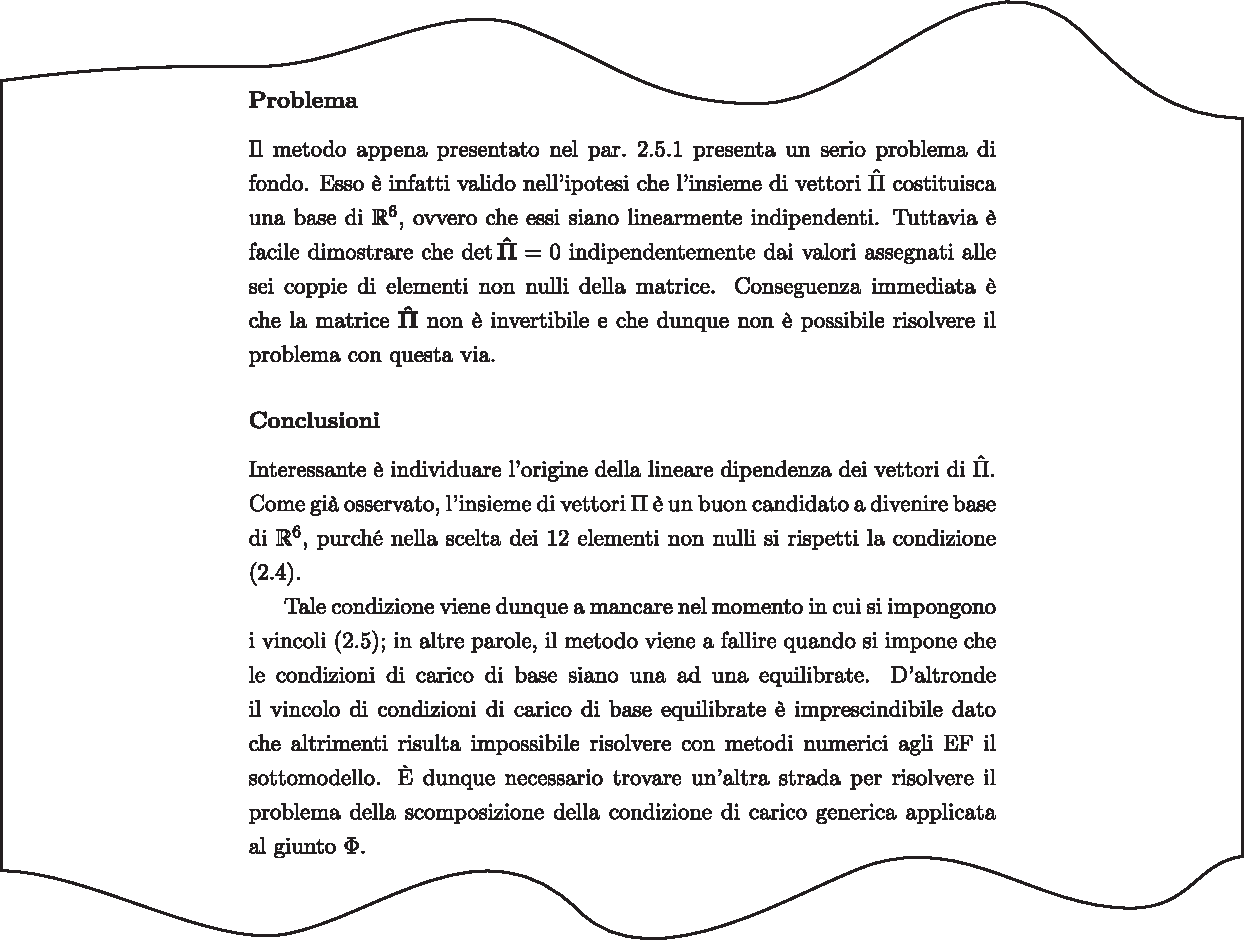
\includegraphics[width=0.85\linewidth]{images/rientro/noindent.pdf}
    \subcaption{Senza pacchetto \ADMpacch{indentfirst}.}\label{fig:rientro:A}
  \end{minipage}%
  \\[0.5cm]
  \begin{minipage}[b]{1.0\linewidth}
    \centering
    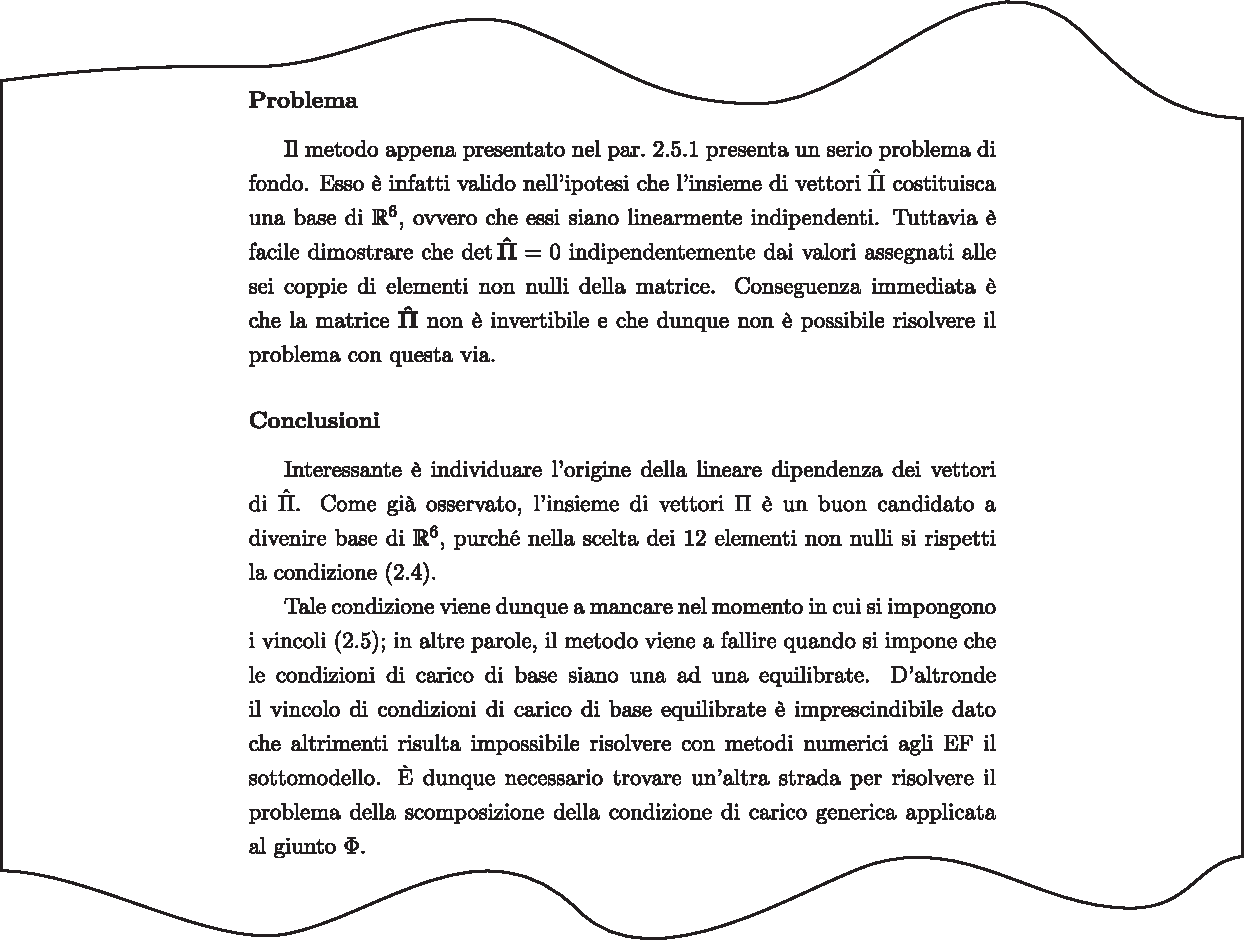
\includegraphics[width=0.85\linewidth]{images/rientro/indent.pdf}
    \subcaption{Con pacchetto \ADMpacch{indentfirst}.}\label{fig:rientro:B}
  \end{minipage}
  \end{tabular}
  \caption{Rientro sulla prima riga.}\label{fig:rientro}
\end{figure*}


\subsection{Caratteri accentati}
\label{sec:accen}

In \LaTeX{} i caratteri accentati possono essere introdotti con i
comandi standard \verb+\`{e}+, \verb+\'{e}+, eccetera, oppure
direttamente da tastiera \verb+è+, \verb+é+, e così via, se nel 
preambolo si carica il pacchetto \ADMpacch{inputenc} con la codifica 
appropriata. 
Si consiglia di caricare il pacchetto con l'opzione \verb+[utf8]+
(si veda il paragrafo~\ref{sec:codifica}).

\section{Il layout}

\subsection{Le testatine ed i piè di pagina}
\label{sec:testatine}

Per personalizzare testatine e piè di pagina è possibile usare il
pacchetto \ADMpacch{fancyhdr}. Per una tesi è probabile che si abbiano
impostazioni differenti a seconda della sezione e dunque è
conveniente definire alcuni comandi personalizzati che modifichino testatine e piè
di pagina; un esempio per \texttt{frontmatter} e \texttt{mainmatter}
potrebbe essere:
\begin{tcblisting}{breakable,
  boxrule=0mm,arc=0mm,boxsep=-7pt,top=9pt,bottom=9pt,oversize,
  listing only,colback=gray!15,
  %listing options={}
}
\newcommand{\fncyfront}{%
    \fancyhead[RO]{{\footnotesize\rightmark}}
    \fancyfoot[RO]{\thepage}
    \fancyhead[LE]{\footnotesize{\leftmark}}
    \fancyfoot[LE]{\thepage}
    \fancyhead[RE,LO]{}
    \fancyfoot[C]{}
    \renewcommand{\headrulewidth}{0.3pt}}
\newcommand{\fncymain}{%
    \fancyhead[RO]{{\footnotesize\rightmark}}
    \fancyfoot[RO]{\thepage}
    \fancyhead[LE]{{\footnotesize\leftmark}}
    \fancyfoot[LE]{\thepage}
    \fancyfoot[C]{}
    \renewcommand{\headrulewidth}{0.3pt}}
\end{tcblisting}

\noindent
da utilizzare nel seguente modo:
\begin{tcblisting}{breakable,
  boxrule=0mm,arc=0mm,boxsep=-7pt,top=9pt,bottom=9pt,oversize,
  listing only,colback=gray!15,
  %listing options={}
}
\pagestyle{fancy}
\fncyfront
\frontmatter
...
\fncymain
\mainmatter
\end{tcblisting}

La definizione di tali comandi è differente a seconda che il testo
sia fronte-retro (\texttt{twoside}) o solo fronte (\texttt{oneside}).

Utilizzando l'opzione \texttt{openright} può capitare di ottenere una pagina
bianca alla fine di un capitolo; per evitare che in questa pagina siano
presenti testatine o piè di pagina, è sufficiente includere nel preambolo
il pacchetto \ADMpacch{emptypage}.

In alternativa a \ADMpacch{fancyhdr} è possibile usare
\ADMpacch{titlesec}. Tale pacchetto ha un'interfaccia d'uso leggermente diversa
da \ADMpacch{fancyhdr} e permette di definire stili diversi da applicarsi in diverse 
parti del documento.

\subsection{Il layout della pagina}

Molto di frequente i regolamenti degli atenei richiedono un layout
della pagina differente da quello prodotto di default dalle classi di
\LaTeX{} ed è dunque necessario modificarlo. Il primo modo per
intervenire è l'utilizzo di comandi interni del \LaTeX{}, quali
\verb+\textwidth+, \verb+\oddsidemargin+, eccetera, tuttavia questa
strada è sconsigliabile per molte ragioni. 

Una migliore soluzione è costituita dal pacchetto 
\ADMpacch{geometry} \citep{umeki:geometry}
che è completamente configurabile. Nel caso che siano necessari degli
interventi locali a pagine o a paragrafi è possibile utilizzare il
pacchetto \ADMpacch{changepage}.

Per rilegare la tesi può essere conveniente indicare sulle pagine
dove tagliare il foglio; questo può essere agevolmente realizzato
utilizzando in coppia i pacchetti \ADMpacch{geometry} e \ADMpacch{crop}. Si
veda ad esempio la figura~\ref{fig:crop}.

\begin{figure*}[tb]
\centering{%
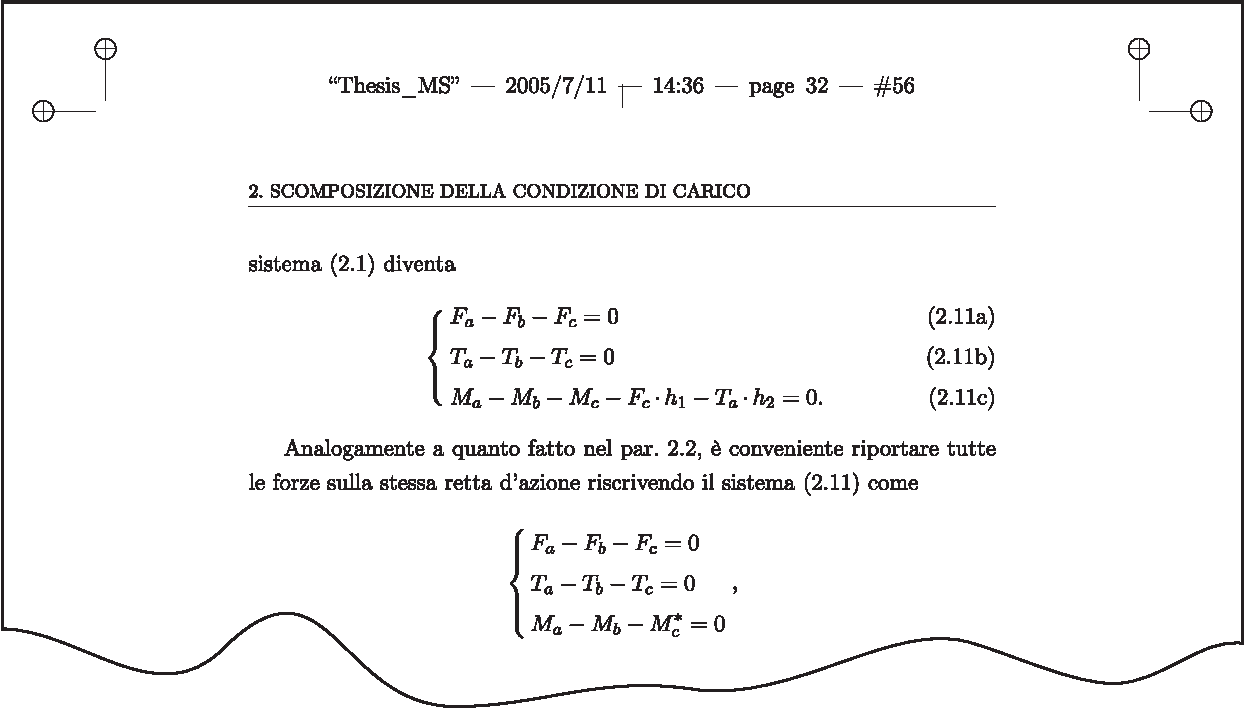
\includegraphics[width=0.90\textwidth]{images/crop/crop.pdf}}
\caption{Esempio di segni per il taglio del foglio.}\label{fig:crop}
\end{figure*}

Di default \LaTeX{} cerca di coprire interamente con il testo o altri elementi
l'intera altezza della pagina e, ove necessario, inserisce degli spazi aggiuntivi tra i
capoversi oppure dilata gli spazi tra le voci degli elenchi puntati e
così via. Se si vuole disattivare questa impostazione ed avere dello
spazio bianco a piè di pagina quando non si riesce a coprirla tutta,
è sufficiente aggiungere nel preambolo il comando
\verb+\raggedbottom+. Il comportamento di default è invece dovuto al
comando \verb+\flushbottom+. Per migliorare la copertura delle pagine
è possibile permettere che siano spezzate le formule matematiche in \emph{display}
aggiungendo al preambolo il comando \verb+\allowdisplaybreaks+
(che funziona solo se è stato caricato il pacchetto \ADMpacch{amsmath}).

\`{E} conveniente non modificare il comportamento di default di
\LaTeX{} fino a quando non si arriva alla versione definitiva del
testo (che precede immediatamente la stampa). Solo in questa fase è
possibile intervenire modificando il posizionamento degli oggetti
flottanti (vedi il paragrafo~\ref{sec:flottanti}), oppure intervenendo con i
comandi appena citati. Prima di modificare le impostazioni di
\LaTeX{} è conveniente provare ad effettuare piccole modifiche al
testo che spesso sono sufficienti per risolvere i problemi e
permettono di ottenere layout più eleganti.

Per approfondimenti sui layout di pagina si consiglia la guida
\emph{Introduzione alla definizione della geometria della pagina}
\citep{beccari:geometria:pagina}.

\subsection{L'interlinea}

Spesso le prescrizioni redazionali impongono un'interlinea diversa da 1.
(valore di default in \LaTeX). Per modificare l'interlinea del
documento esistono più strade, tuttavia la più indicata consiste nel 
caricare il pacchetto \ADMpacch{setspace}. Tale pacchetto fornisce tre 
interlinee predefinite richiamate con i comandi \verb+\singlespacing+ (interlinea singola),
\verb+\onehalfspacing+ (interlinea 1,5) e \verb+\doublespacing+
(interlinea doppia). Se è necessaria un'interlinea differente, è
sufficiente utilizzare il comando \verb+\linespread{...}+ mettendo tra
parentesi graffe il numero che rappresenta il fattore di scala per
l'avanzamento di riga.

\section{Lo stile}

\begin{figure*}[tb]
\centering{%
\includegraphics[width=0.90\textwidth]{images/cambria/cambria.pdf}}
\caption{Esempio d'uso dei font Calibri per il testo e Cambria Math per la matematica.}\label{fig:cambria}
\end{figure*}


\subsection{I font}

In primo luogo, lavorando con \verb+pdflatex+, è consigliabile utilizzare l'encoding T1 che
rappresenta lo standard di codifica dei caratteri di \LaTeX{}.
Tale codifica è attivata nel preambolo per mezzo del comando
\begin{tcblisting}{breakable,
  boxrule=0mm,arc=0mm,boxsep=-7pt,top=9pt,bottom=9pt,oversize,
  listing only,colback=gray!15,
  %listing options={}
}
\usepackage[T1]{fontenc}
\end{tcblisting}

Se la tesi è di tipo scientifico, è conveniente abilitare i font matematici 
forniti dall'\AmS{} (American Mathematical Society) con il comando
\begin{tcblisting}{breakable,
  boxrule=0mm,arc=0mm,boxsep=-7pt,top=9pt,bottom=9pt,oversize,
  listing only,colback=gray!15,
  %listing options={}
}
\usepackage{amssymb}
\end{tcblisting}

\noindent
Il pacchetto \ADMpacch{amssymb} carica il pacchetto \ADMpacch{amsfonts}
e definisce i comandi per usare i simboli introdotti da quest'ultimo.

Per la matematica conviene in generale aggiungere il comando
\begin{tcblisting}{breakable,
  boxrule=0mm,arc=0mm,boxsep=-7pt,top=9pt,bottom=9pt,oversize,
  listing only,colback=gray!15,
  %listing options={}
}
\usepackage{mathtools}
\end{tcblisting}

\noindent
che carica anche il pacchetto \ADMpacch{amsmath} e fornisce svariate estensioni 
per il miglioramento della struttura informativa e della stampa di documenti 
che contengono formule matematiche. 

Per modificare la dimensione del font, in aggiunta ai
comandi standard,\footnote{\texttt{tiny}, \texttt{scriptsize},
\texttt{footnotesize}, \texttt{small}, \texttt{normalsize},
\texttt{large}, \texttt{Large}, \texttt{LARGE}, \texttt{huge} e
\texttt{Huge}.} è utile il pacchetto \ADMpacch{relsize} che consente di
assegnare dimensioni relative con i comandi \verb+\smaller+ e
\verb+\larger+.

Riguardo al tipo di font da utilizzare,
l'esperienza conferma che, quasi certamente, la scelta migliore è quella di 
usare i font che \LaTeX\ carica di default, ovvero la famiglia Computer Modern
sviluppata dallo stesso inventore del {\TeX}, Donald Knuth. 
Questi caratteri possono essere usati nella variante Latin Modern
prodotto dal \textsc{gust} (gruppo utenti di \TeX{} polacco)%
\footnote{\url{http://www.gust.org.pl/projects/e-foundry/latin-modern}}
caricando il pacchetto \ADMpacch{lmodern}:
\begin{tcblisting}{breakable,
  boxrule=0mm,arc=0mm,boxsep=-7pt,top=9pt,bottom=9pt,oversize,
  listing only,colback=gray!15,
  %listing options={}
}
\usepackage[T1]{fontenc}
\usepackage{lmodern}
\end{tcblisting}

Se si vuole a tutti i costi cambiare font, è bene ricordare che è
necessario scegliere quattro famiglie (Serif, \textsf{Sans-serif},
\texttt{Typewriter} e i font per la matematica) che formino una buona
combinazione. A tale proposito, è importante ricordare che i font,
tranne alcune eccezioni,\footnote{Il gruppo utenti \TeX{} danese ospita una pagina in
cui sono riportati tutti i font che supportano la matematica:
\url{http://www.tug.dk/FontCatalogue/mathfonts.html}.} non hanno
tutti i simboli necessari per la matematica e quindi non possono
essere usati se non nel testo. 

Per cambiare font è possibile caricare uno dei numerosi pacchetti dedicati. 
Un elenco dei font disponibili e i pacchetti da caricare per usarli è riportato 
sul sito del gruppo di utenti \TeX{} danese.\footnote{\url{http://www.tug.dk/FontCatalogue}}

Un'ottima alternativa ai caratteri di default è offerta dai pacchetti 
\ADMpacch{newtxtext} e \ADMpacch{newtxmath}.
Con essi si caricano: il font Times (o un suo clone) per il testo, un font appositamente disegnato
per la matematica basato su Times Italic, un clone del font Helvetica per la famiglia sans serif, 
vari possibili font per la famiglia typewriter.

Parlando qui di font, non si può fare a meno di menzionare un'importante alternativa al programma
\verb+pdflatex+, cioè \verb+xelatex+ o anche \XeLaTeX{}.
La caratteristica principale di \XeLaTeX{} è che può adoperare senza bisogno di 
installazioni particolari tutti i font noti al sistema operativo in uso, 
che siano in formato OpenType o TrueType. 
Questi font sono dotati di tabelle interne con cui \XeLaTeX{} è capace di creare 
al volo la struttura dati che nel \TeX{} tradizionale risiede in particolari file
metrici (\verb+.tfm+). 
Altra importante caratteristica di \XeLaTeX{} è che lavora direttamente con file 
in codifica Unicode, cioè UTF-8 oppure UTF-16.
Un esempio di sorgente con caratteri speciali è il seguente:

\begin{tcblisting}{breakable,
  boxrule=0mm,arc=0mm,boxsep=-7pt,top=9pt,bottom=9pt,oversize,
  listing only,colback=gray!15,
  %listing options={}
}
\documentclass{article} 

\usepackage{fontspec}
\usepackage{unicode-math}
\setmainfont{Calibri}
\setmathfont{Cambria Math}

\begin{document}
äöüß
\[
c = \sqrt{\frac{E}{m}}
\]
The Bezier curve $C$ of degree $m$ is
\[
C(u) = \sum_{i=0}^m f_i(u)P_i
\]
\end{document}
\end{tcblisting}

\noindent
Questo sorgente produce un output come quello della figura~\ref{fig:cambria}
in cui si nota l'uso del font Calibri per il testo e del font Cambria Math per la matematica.

Per una introduzione all'uso di \XeLaTeX{} si rimanda alla
guida di \citet{gregorio:xelatex} e ai riferimenti in essa contenuti.



\subsection{Il titolo dei capitoli}

Per personalizzare il formato dei titoli dei capitoli è possibile
utilizzare il pacchetto \ADMpacch{fncychap}; si rimanda a \citet{art:mori:tesi}
per maggiori dettagli.

Nella figura~\ref{fig:Titoli} è mostrato un esempio di personalizzazione
attraverso il pacchetto \ADMpacch{titlesec}.
Una volta definito lo stile nel preambolo con il comando \verb+\titleformat+
la formattazione del titolo del capitolo è ottenuta semplicemente nel documento 
attraverso il comando standard della classe \verb+book+:
\begin{tcblisting}{breakable,
  boxrule=0mm,arc=0mm,boxsep=-7pt,top=9pt,bottom=9pt,oversize,
  listing only,colback=gray!15,
  %listing options={}
}
\chapter{Definizioni di base e notazioni} 
\end{tcblisting}

\clearpage


\begin{figure*}[p]
\centering
\begin{minipage}[b]{\linewidth}
\begin{tcblisting}{breakable,
  boxrule=0mm,arc=0mm,boxsep=-7pt,top=9pt,bottom=9pt,oversize,
  listing only,colback=gray!15,
  %listing options={}
}
\usepackage[calcwidth,pagestyles]{titlesec}% loads titleps 
\usepackage{adjustbox,xcolor}

% chapter head style via titlesec
\titleformat{\chapter}[display]
    {\bfseries\Large}
    {\color{blue!65!black}\filleft%
        \minsizebox{!}{24pt}{\chaptertitlename}% needs package adjustbox
        \lapbox[0pt]{\width}{%
            \minsizebox{!}{40pt}{%
                \ \colorbox{blue!65!black}{\color{white}\thechapter}% needs xcolor
            }%
        }% needs package adjustbox
    }
    {4ex}
    {{\color{blue!65!black}\titlerule}
        \huge\bfseries\scshape
        \vspace{2ex}%
        \filright}
    [\vspace{2ex}%
        {\color{blue!65!black}\titlerule}]
\end{tcblisting}
\end{minipage}
\\[0.3cm]
\fbox{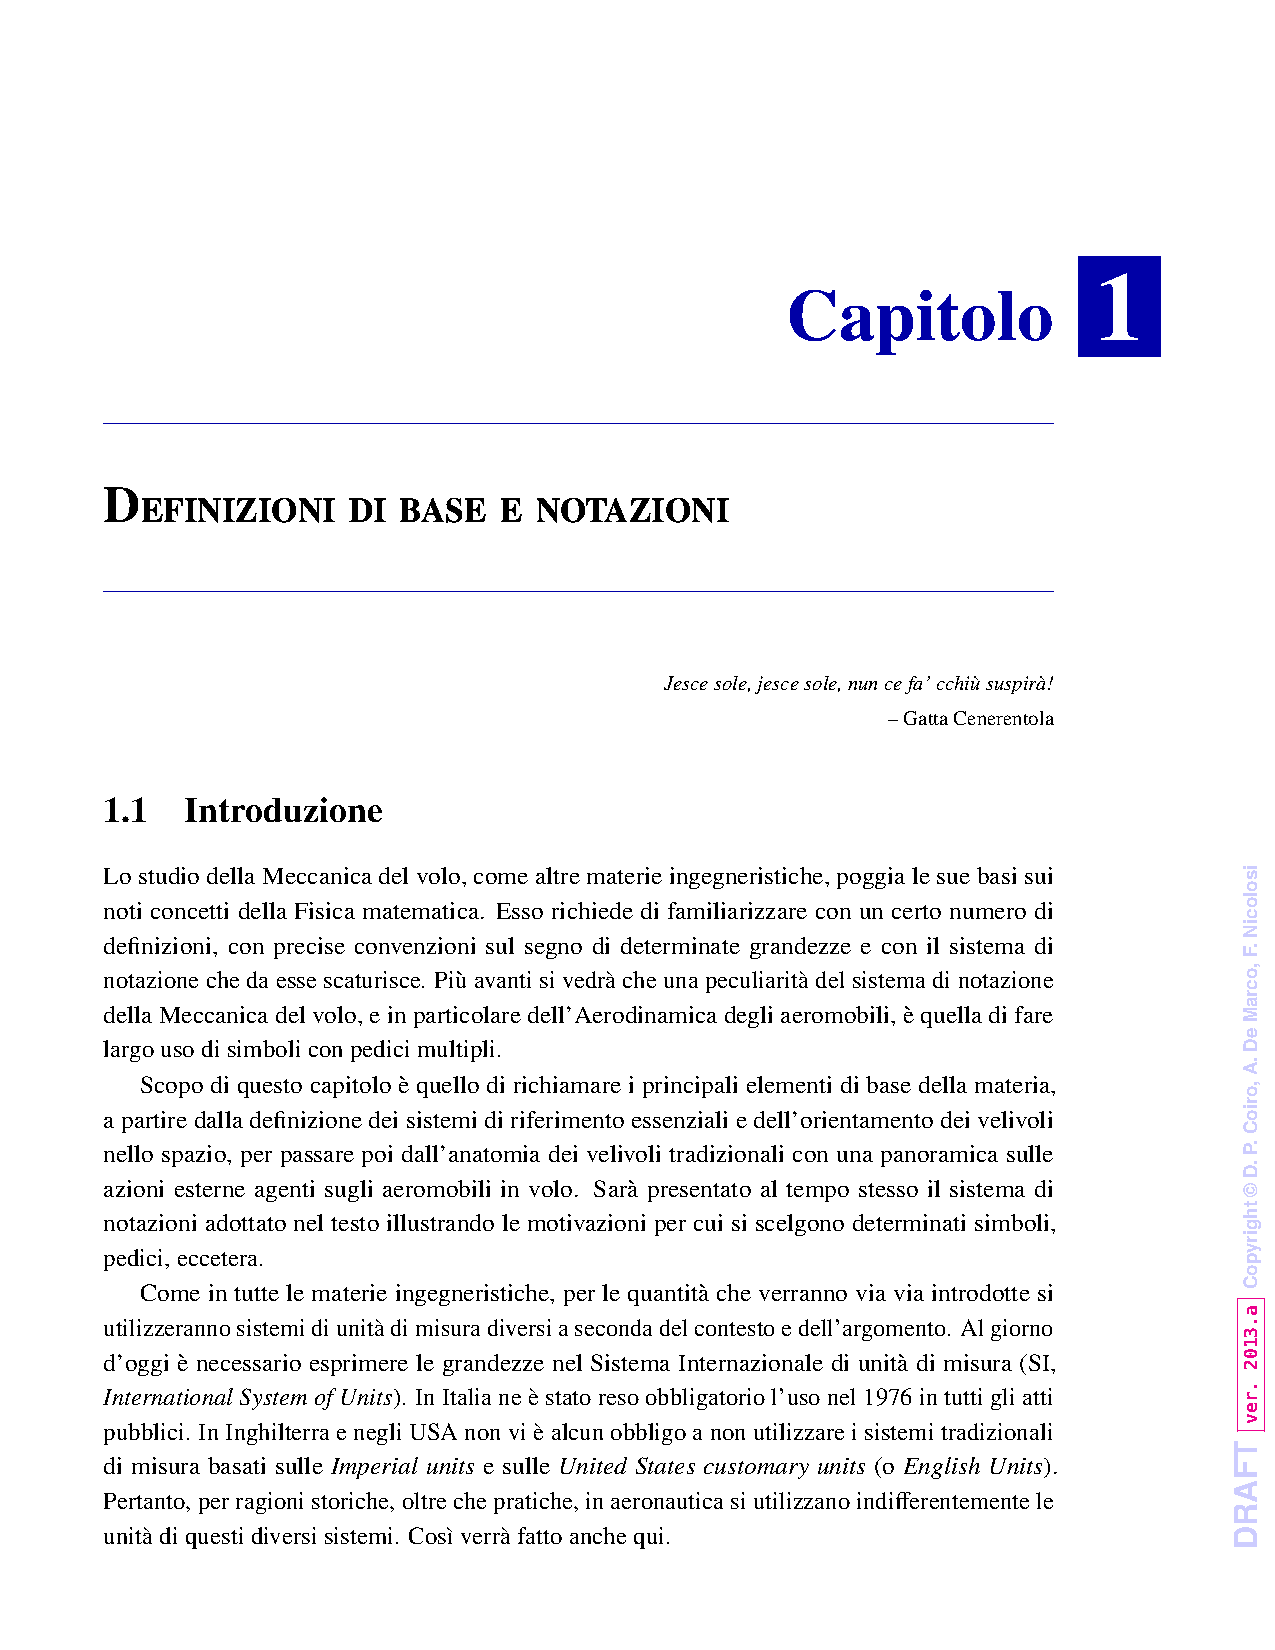
\includegraphics[height=0.45\textheight]{images/titolo/titolo.pdf}}
\caption[Esempio di definizione del titolo dei capitoli con \texorpdfstring{\ADMpacch}{}{titlesec}]{Esempio di definizione del titolo dei capitoli con \ADMpacch{titlesec}.
  Il comando standard \texttt{\string\chapter} della classe \class{book} produce un titolo
  nel formato personalizzato.}\label{fig:Titoli}
\end{figure*}


\subsection{Liste}

%\noindent
Per personalizzare i tre ambienti standard dedicati alle liste,
cioè \verb+enumerate+, \verb+itemize+ e \verb+description+,
ci consiglia il pacchetto \ADMpacch{enumitem}.



\subsection{I ``mini indici''}

Quando i capitoli hanno una struttura particolarmente complessa, può
essere conveniente riportare nella pagina iniziale l'indice del
capitolo (vedi ad esempio la figura~\ref{fig:mini}). Questi ``mini
indici'' possono essere prodotti automaticamente con il pacchetto
\ADMpacch{minitoc}.

\begin{figure*}[tb]
\centering{%
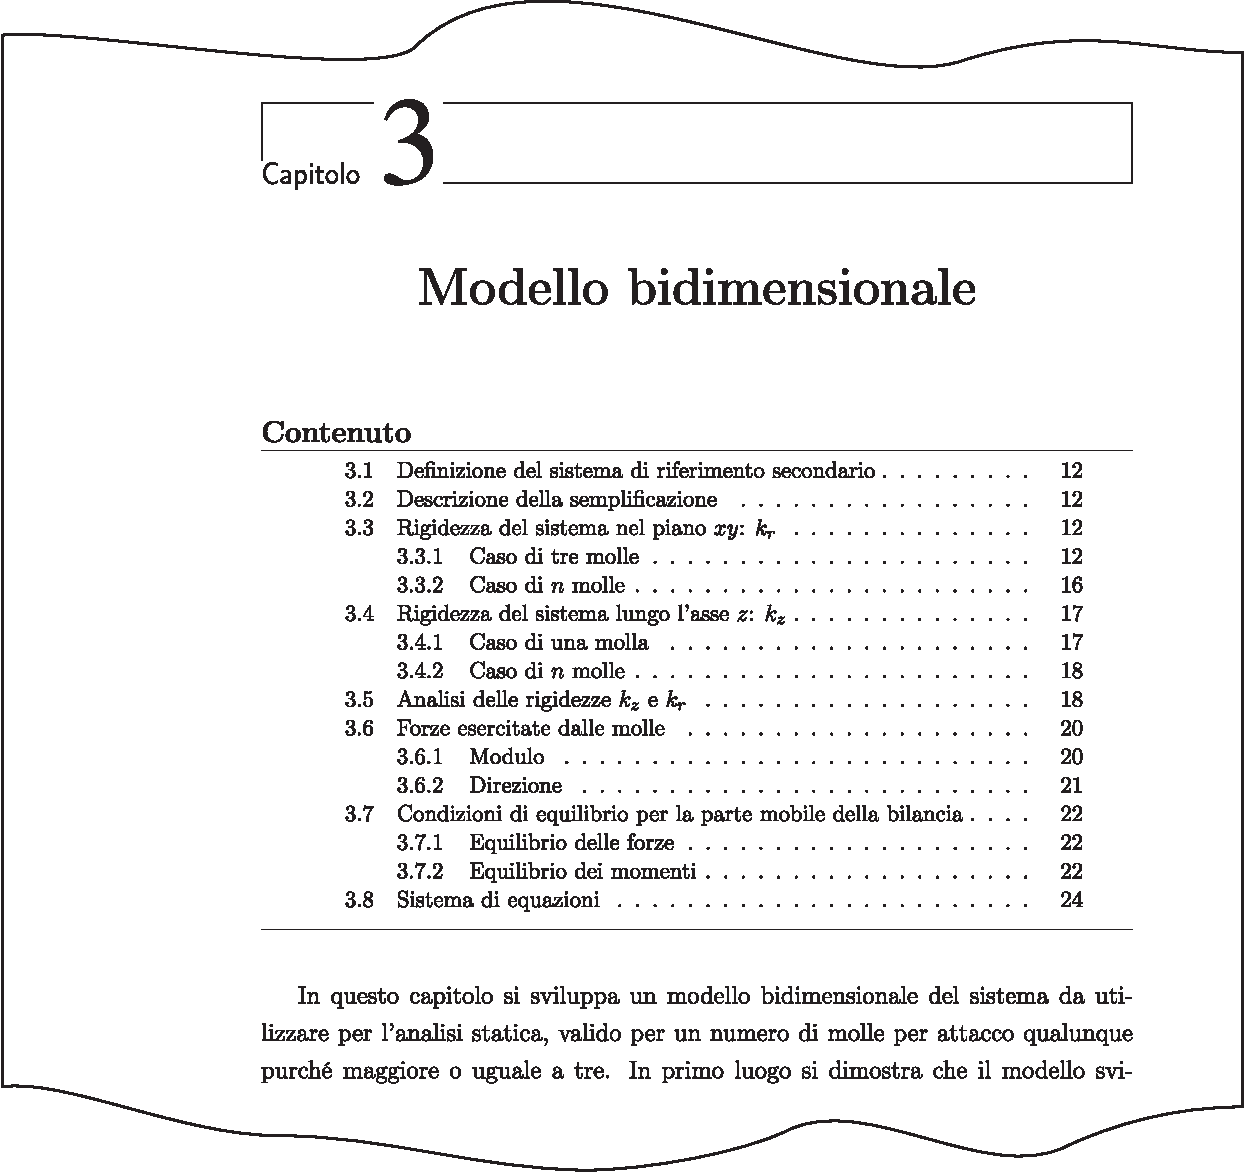
\includegraphics[width=0.8\textwidth]{images/mini/mini.pdf}}
\caption{Esempio di ``mini indice''.}\label{fig:mini}
\end{figure*}

%
\subsection{Le epigrafi}

Talvolta si vogliono inserire epigrafi nella pagina iniziale dei
capitoli. Per farlo è possibile utilizzare il pacchetto
\ADMpacch{epigraph}; un esempio è riportato nella figura~\ref{fig:epig}.

\begin{figure*}[tb]
\centering{%
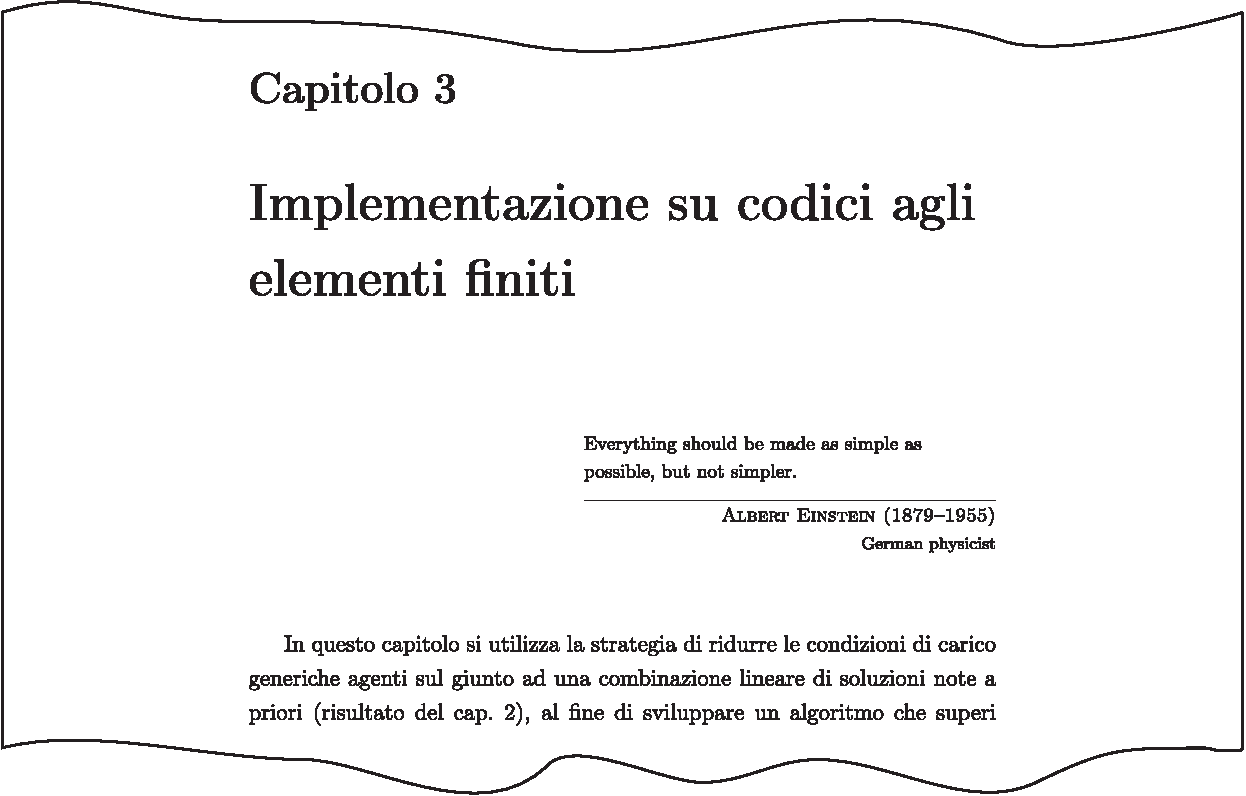
\includegraphics[width=0.85\textwidth]{images/epig/epig.pdf}}
\caption{Esempio di epigrafe.}\label{fig:epig}
\end{figure*}


\subsection{Le note}

\LaTeX{} produce di default un layout delle note di alta qualità;
esistono tuttavia alcuni accorgimenti per modificarlo, quando lo si
ritenga strettamente necessario. Il pacchetto \ADMpacch{footmisc}
fornisce molti controlli sulle note tra cui la possibilità di forzare
le note al fondo della pagina\footnote{Normalmente \LaTeX{} unisce
le note con l'ultima riga della pagina e dunque su pagine non piene
non si hanno le note a fondo pagina.} con l'opzione \texttt{bottom};
si veda la figura~\ref{fig:note}.

\begin{figure*}[tb]
  \centering
  \begin{tabular}{@{}c@{}}
  \begin{minipage}[b]{1.0\linewidth}
    \centering
    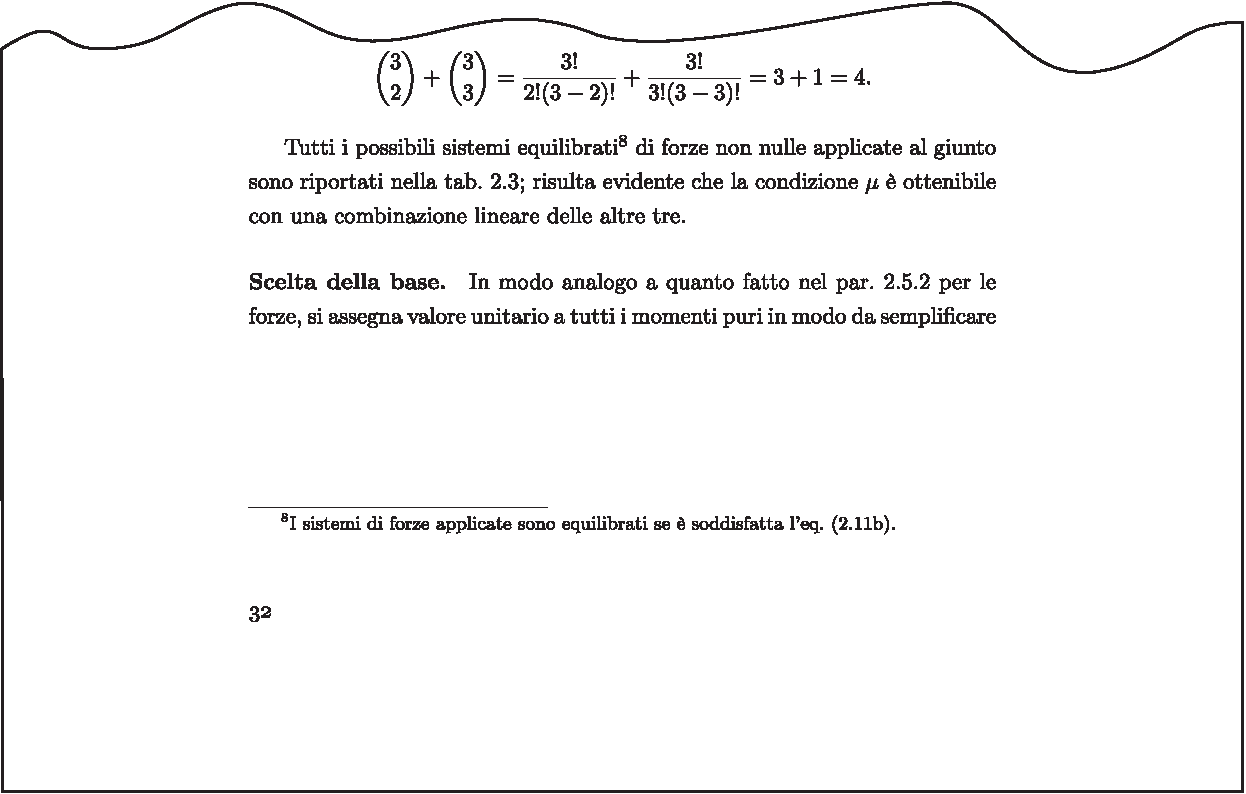
\includegraphics[width=0.75\linewidth]{images/note/notabo.pdf}
    \subcaption{con opzione \texttt{bottom}}\label{fig:note:A}
  \end{minipage}%
  \\
  \begin{minipage}[b]{1.0\linewidth}
    \centering
    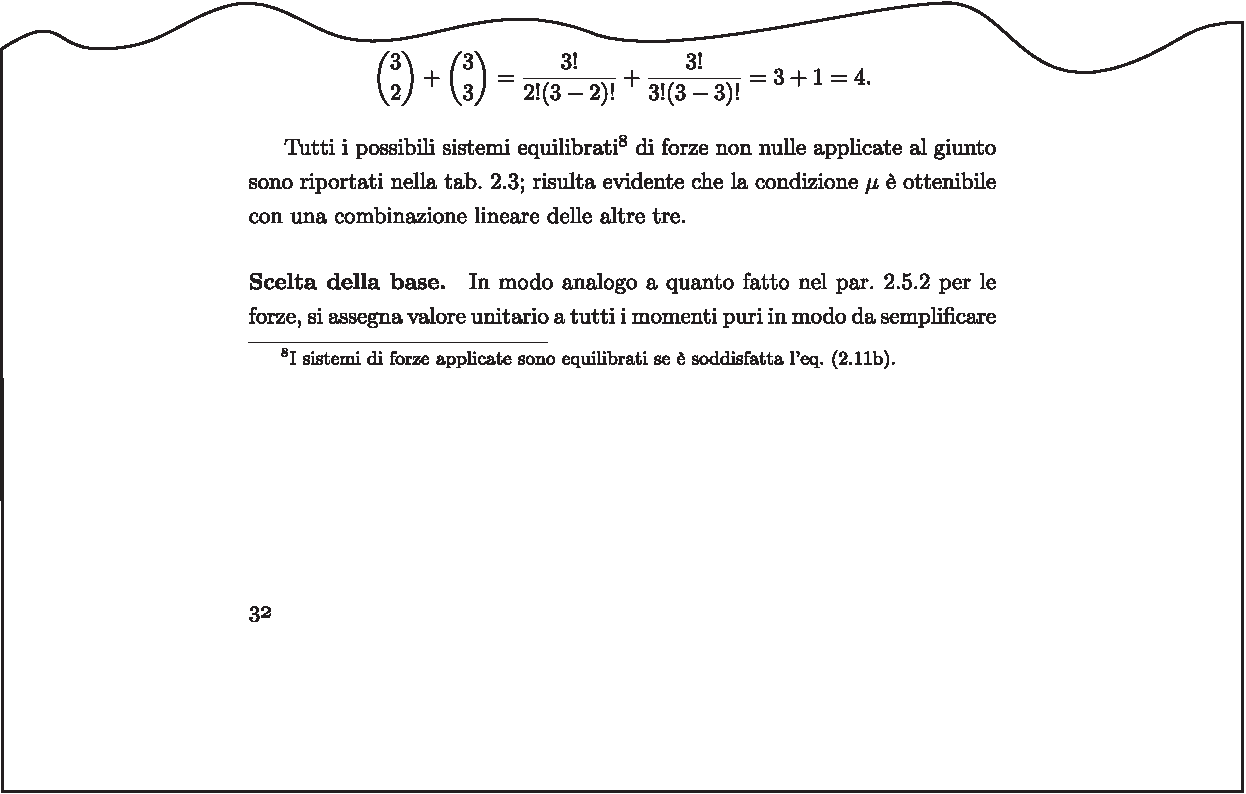
\includegraphics[width=0.75\linewidth]{images/note/notanobo.pdf}
    \subcaption{senza opzione \texttt{bottom}}\label{fig:note:B}
  \end{minipage}
  \end{tabular}
  \caption{Posizione delle note.}\label{fig:note}
\end{figure*}

Per impedire che le note vengano spezzate su più pagine è sufficiente
assegnare al parametro di penalità un valore molto elevato, ad
esempio
\begin{tcblisting}{breakable,
  boxrule=0mm,arc=0mm,boxsep=-7pt,top=9pt,bottom=9pt,oversize,
  listing only,colback=gray!15,
  %listing options={}
}
\interfootnotelinepenalty=10000
\end{tcblisting}

\noindent
mentre per controllare la dimensione della zona assegnata alle note a
piè di pagina si può usare il comando
\begin{tcblisting}{breakable,
  boxrule=0mm,arc=0mm,boxsep=-7pt,top=9pt,bottom=9pt,oversize,
  listing only,colback=gray!15,
  %listing options={}
}
\dimen\footins=2cm
\end{tcblisting}

\section{La matematica}

Si consiglia il lettore di consultare l'\emph{Arte} di \citeauthor{man:Pantieri}, la
guida del \citet{beccari:guida:guit} e la guida di \citet{misc:mathmode}
per approfondimenti sulla scrittura matematica (semplice e avanzata) in \LaTeX{}.
Qui di seguito si accenna ad alcuni aspetti interessanti per chi scrive una tesi di laurea.

\subsection{I simboli ``speciali''}

Intendendo con ``simboli speciali'' tutti quelli che non sono
inseribili direttamente dalla tastiera, è necessario distinguere tra
quelli matematici e quelli non matematici: per i primi dovrebbe
essere sufficiente caricare i simboli dell'\AmS{} con il pacchetto
\ADMpacch{amssymb}; per tutti gli altri simboli sono necessari pacchetti
appositi che possono essere facilmente identificati consultando la preziosa
guida \emph{The comprehensive \LaTeX{} symbol list} \citep{man:ltxsymbols}.

\subsection{Rappresentazione dei numeri}

Un pacchetto molto utile per la rappresentazione di numeri è
\ADMpacch{numprint}. Tra le funzioni di tale pacchetto si ricordano
l'inserimento di un separatore ogni tre cifre per le migliaia e
l'approssimazione automatica. Ad esempio
\begin{tcblisting}{breakable,
  boxrule=0mm,arc=0mm,boxsep=-7pt,top=9pt,bottom=9pt,oversize,
  listing only,colback=gray!15,
  %listing options={}
}
\numprint{2.742647826672E-01}
\end{tcblisting}

\noindent
produce

%\esempio{$2,743\cdot 10^{-01}$}
\noindent
\adjustbox{center=\linewidth}{
  $\num[round-precision=3]{2{,}743}\cdot 10^{-01}$
}

\subsection{Unità di misura}

Le unità di misura del Sistema Internazionale possono essere inserite con i comandi
del pacchetto \ADMpacch{siunitx} (se ne veda la documentazione), che permette di regolarne
molto finemente il formato e di cambiare il risultato nel documento
finito operando un'unica modifica nel preambolo anziché agire a mano su
ciascuna unità di misura.
Dato che le convenzioni tipografiche italiane prevedono la virgola e non
il punto (predefinito dal pacchetto) come separatore decimale, il pacchetto
va caricato almeno con l'opzione seguente:
\begin{tcblisting}{breakable,
  boxrule=0mm,arc=0mm,boxsep=-7pt,top=9pt,bottom=9pt,oversize,
  listing only,colback=gray!15,
  %listing options={}
}
\usepackage[output-decimal-marker={,}
  % ... altre opzioni
  ]{siunitx}
\end{tcblisting}

I comandi fondamentali sono \verb+\num+ (simile a \verb+numprint+), \verb+\SI+ e \verb+\si+ 
che permettono di formattare i numeri, le grandezze fisiche e le unità di misura in maniera 
configurabile.

Il pacchetto dispone di un modulo di elaborazione dei numeri che
consente di avere nei sorgenti dei valori numerici del tipo \verb+30e3+ che le macro di 
scrittura trasformano in $30\times 10^3$. Questo permette di trarre i valori numerici da 
file scritti dagli stessi strumenti di misura moderni, dove i numeri sono espressi con 
la notazione informatica dei numeri a virgola mobile. 

Si può specificare il numero di cifre da scrivere nei valori numerici delle misure: 
il modulo di elaborazione dei numeri provvede ad arrotondare quel valore numerico al 
numero richiesto di decimali.
Infatti se si specifica che si vogliono consistentemente 4 decimali e la virgola
decimale, il numero \verb+1.234567+, con il comando
\begin{tcblisting}{breakable,
  boxrule=0mm,arc=0mm,boxsep=-7pt,top=9pt,bottom=9pt,oversize,
  listing only,colback=gray!15,
  %listing options={}
}
|\color{green!40!black}\relsize{-1}\itshape nel preambolo|
\sisetup{
  round-mode      = places,
  round-precision = 4
}

|\color{green!40!black}\relsize{-1}\itshape nel testo|
\num{1.234567}
\end{tcblisting}

\noindent
viene stampato nella forma 

\noindent
\adjustbox{center=\linewidth}{
  \num[round-mode=places,round-precision=4]{1.234567}
}

\noindent
dove il numero di decimali è quello voluto ma l'ultima cifra tiene conto dell'arrotondamento in
alto, visto che la parte scartata è maggiore della metà dell'unità corrispondente
all'ultima cifra scritta; inoltre il punto decimale è consistentemente cambiato
nella virgola, come richiesto.

Il seguente frammento di codice:
\begin{tcblisting}{breakable,
  boxrule=0mm,arc=0mm,boxsep=-7pt,top=9pt,bottom=9pt,oversize,
  listing only,colback=gray!15,
  %listing options={}
}
\SI{23.4}{kg.m.s^{-2}} \\
$r=\SI{0,8768(11)e-15}{m}$ \\
\|\color{blue!60!black}\sffamily\bfseries si|{\joule\per\mole\per\kelvin}\\
\|\color{blue!60!black}\sffamily\bfseries si|{J.mol^{-1}.K^{-1}}\\
\SI{100}{\celsius} \\
\ang{1;2;3}
\end{tcblisting}

\noindent
produce la di scrittura di grandezze fisiche nella forma:

\smallskip
\noindent
\centerline{%
\adjustbox{minipage=0.7\linewidth}{
  \SI[round-precision=1]{23.4}{kg.m.s^{-2}} \\[2pt]
  $r=\SI{0,8768(11)e-15}{m}$ \\[2pt]
  \si{\joule\per\mole\per\kelvin}\\[2pt]
  \si{J.mol^{-1}.K^{-1}}\\[2pt]
  \SI{100}{\celsius} \\[2pt]
  \ang{1;2;3}
}
}% end of \centerline

\subsection{Altri pacchetti}

Per evidenziare gli ambienti matematici può essere utilizzato il
pacchetto \ADMpacch{empheq}. 
Il seguente risultato:
\begin{empheq}[box=\fbox]{align}
f(x) & = a x + b \\
E & = mc^2 + \int_0^T f(t) \ADMdiff{t}
\end{empheq}

\noindent
è prodotto con il codice:

\begin{tcblisting}{breakable,
  boxrule=0mm,arc=0mm,boxsep=-7pt,top=9pt,bottom=9pt,oversize,
  listing only,colback=gray!15,
  %listing options={}
}
|\color{green!40!black}\relsize{-1}\itshape nel preambolo|
\usepackage{empheq}
\newcommand*{\diff}{\mathop{}\!\mathrm{d}}

|\color{green!40!black}\relsize{-1}\itshape nel testo|
\begin{empheq}[box=\fbox]{align}
f(x) & = a x + b \\
E & = mc^2 + \int_0^T f(t)\, \diff{t}
\end{empheq}
\end{tcblisting}

\noindent
Si noti la definizione del comando \verb+\diff+ per il simbolo di differenziale: 
in ambiente matematico \verb+\diff{t}+ permette di ottenere `$\mathrm{d}t$'
come richiesto dalle norme
\citet{man:ISO:math:symbols}.


Per la personalizzazione degli ambienti
``tipo teorema'' è necessario il pacchetto \ADMpacch{ntheorem}. Il
pacchetto \ADMpacch{xfrac} permette invece di scrivere correttamente le
frazioni nel testo e nel testo matematico (ad esempio: \sfrac{5}{7}).

\section{Codici ed algoritmi}

Il pacchetto \ADMpacch{listings} è un potente strumento con il quale si
gestisce la scrittura di codici in numerosi linguaggi di programmazione, controllandone
molto finemente il formato.

{\tolerance=3000 Per la formattazione di algoritmi sono invece consigliabili i
pacchetti \ADMpacch{algorithm} e \ADMpacch{algpseudocode}: il primo
genera degli oggetti flottanti mentre il secondo no.\par}

\section{Riferimenti incrociati}

In molti casi è comodo usare contemporaneamente i comandi \verb+\ref+
e \verb+\pageref+ per riferirsi a figure e tabelle, specialmente
quando ci sono più pagine tra il riferimento e l'oggetto. Per questo,
alcuni utenti utilizzano comandi come
\begin{tcblisting}{breakable,
  boxrule=0mm,arc=0mm,boxsep=-7pt,top=9pt,bottom=9pt,oversize,
  listing only,colback=gray!15,
  %listing options={}
}
\newcommand{\fullref}[1]{%
    \ref{#1} a pagina~\pageref{#1}}
\end{tcblisting}

\noindent
che semplifica la scrittura del riferimento. Tuttavia, non sapendo a
priori dove sia posizionato l'oggetto a cui ci si riferisce,
utilizzando un comando del genere può capitare che il \verb+\pageref+
punti alla pagina stessa dove si trova il riferimento producendo un
risultato insoddisfacente.

Per rendere automatica la scrittura dei riferimenti completi è
possibile utilizzare il pacchetto \ADMpacch{varioref} che introduce il
comando \verb+\vref+ da usarsi nello stesso modo del comune
\verb+\ref+. Tale pacchetto funziona in parallelo a \ADMpacch{babel} e
quindi si adatta alla lingua utilizzata nel testo. Ad esempio
\begin{tcblisting}{breakable,
  boxrule=0mm,arc=0mm,boxsep=-7pt,top=9pt,bottom=9pt,oversize,
  listing only,colback=gray!15,
  %listing options={}
}
si veda la figura~\vref{fig:Mia:Figura}
\end{tcblisting}

\noindent
produce, a seconda di dove viene posizionata la figura, qualcosa del
tipo 

\smallskip
\noindent
\centerline{%
\adjustbox{center=1.0\linewidth}{
  si veda la figura~3.1 nella pagina successiva
}
}% end of \centerline

\smallskip
\noindent
oppure

\smallskip
\noindent
\centerline{%
\adjustbox{center=1.0\linewidth}{
  si veda la figura~3.1 a pagina 24
}
}% end of \centerline

Per quanto riguarda invece il riferimento ad equazioni, è
consigliabile utilizzare il comando \verb+\eqref{...}+ di \ADMpacch{amsmath} al posto di
\verb+(\ref{...})+. Ad esempio
\begin{tcblisting}{breakable,
  boxrule=0mm,arc=0mm,boxsep=-7pt,top=9pt,bottom=9pt,oversize,
  listing only,colback=gray!15,
  %listing options={}
}
... grazie all'equazione~\eqref{e2}
\end{tcblisting}

\smallskip
\noindent
produce qualcosa del tipo 

\medskip
\noindent
\centerline{%
\adjustbox{minipage=0.9\linewidth}{
  \ldots\ grazie all'equazione~(3.6)
}
}% end of \centerline

\medskip
Un pacchetto alternativo e per certi aspetti più potente di \ADMpacch{varioref} è il
pacchetto \ADMpacch{cleveref}. Si rimanda il lettore al manuale d'uso per approfondimenti.

\section{Revisione del codice}

In fase di revisione del codice è molto utile, oltre ad un'attenta
lettura del file di \emph{log} dei messaggi (\texttt{.log}), l'utilizzo dei pacchetti
\ADMpacch{refcheck} e \ADMpacch{showkeys} che controllano l'utilizzo dei
\verb+\label+ e dei \verb+\ref+. In aggiunta a questi è anche
conveniente abilitare l'opzione \texttt{draft} per la
\texttt{documentclass}: in questo modo i punti in cui il testo esce 
dai margini verranno evidenziati con delle barre nere.

\chapter{Siti utili}
\label{sec:siti:utili}

In aggiunta alle guide ed ai manuali citati nella bibliografia, sono disponibili 
sul Web una serie di risorse utili per risolvere i problemi incontrati durante
l'utilizzo di \LaTeX.

Il riferimento primario per la comunità italiana di utenti \LaTeX\ è il
sito del \guit\ (Gruppo Italiano degli Utenti di \TeX\ e \LaTeX)\footnote{\url{http://www.guitex.org}} che ospita un forum sull'argomento.\footnote{\url{http://www.guitex.org/home/it/forum/index}} sed ha anche una sezione documentazione ben organizzata.

Altro sito di interesse è quello del
%costituito da the Comprehensive TeX Archive Network 
\textsc{ctan}
%\footnote{\url{http://www.ctan.org}} 
che ospita gran parte del materiale su \LaTeX\ disponibile in rete ed è dotato di un
motore di ricerca.

Sarovar\footnote{\url{http://texcatalogue.sarovar.org}} è un
catalogo molto completo di pacchetti e programmi legati a \TeX\ e
\LaTeX. Permette svariati tipi di ricerca, in particolare è
estremamente utile la lista ``topical'' quando non si conosce il nome
di un pacchetto ma solo ``quello che deve fare''.

Altri due importanti riferimenti sono il sito di domande e risposte
su StackExchange\footnote{\url{http://tex.stackexchange.com}}
e il sito \LaTeX{} Community.\footnote{\url{http://www.latex-community.org}}

\chapter{Strumenti per la compilazione \emph{in the cloud}}
\label{sec:siti:compilazione:online}

Nel panorama degli strumenti per \LaTeX{} si è recentemente affermata una nuova
possibilità di lavoro. Diversamente dal metodo tradizionale in cui si produce un 
documento tramite un sistema \TeX{} installato sul proprio computer,
oggi esistono siti internet che permettono la compilazione online di documenti \LaTeX{}
residenti in una \emph{cloud} dedicata.
Alcuni chiamano queste applicazioni web col nome di strumenti di compilazione 
\emph{in the cloud}.\footnote{Si veda anche \url{http://en.wikibooks.org/wiki/LaTeX/Collaborative_Writing_of_LaTeX_Documents}}
Essi sono inoltre adatti alla stesura `collaborativa' di documenti, cioè per i quali le modifiche
online sono consentite a più utenti; la gestione incrementale delle modifiche è una delle 
funzionalità offerte.

Alcuni esempi sono (figura~\ref{fig:Online:Tools}):
%\begin{compactitemize}
\begin{itemize}
\item
ShareLaTeX: \url{https://www.sharelatex.com}
\item
writeLaTeX: \url{https://www.writelatex.com}
\item
verbosus: \url{https://verbosus.com}
\item
Authorea: \url{https://www.authorea.com}
\end{itemize}
%\end{compactitemize}

Il servizio offerto da questi siti per la gestione dei progetti \LaTeX{}
presenta diversi profili possibili. Tipicamente vi è sempre la possibilità
di registrarsi gratuitamente avendo a disposizione un limitato spazio di 
memorizzazione e un limitato numero di collaboratori.

\begin{figure*}[p]
\centering
\begin{tabular}{@{}c@{}}
\begin{minipage}[b]{\linewidth}
  \centering
  \url{https://www.sharelatex.com}\\[4pt]
  \fbox{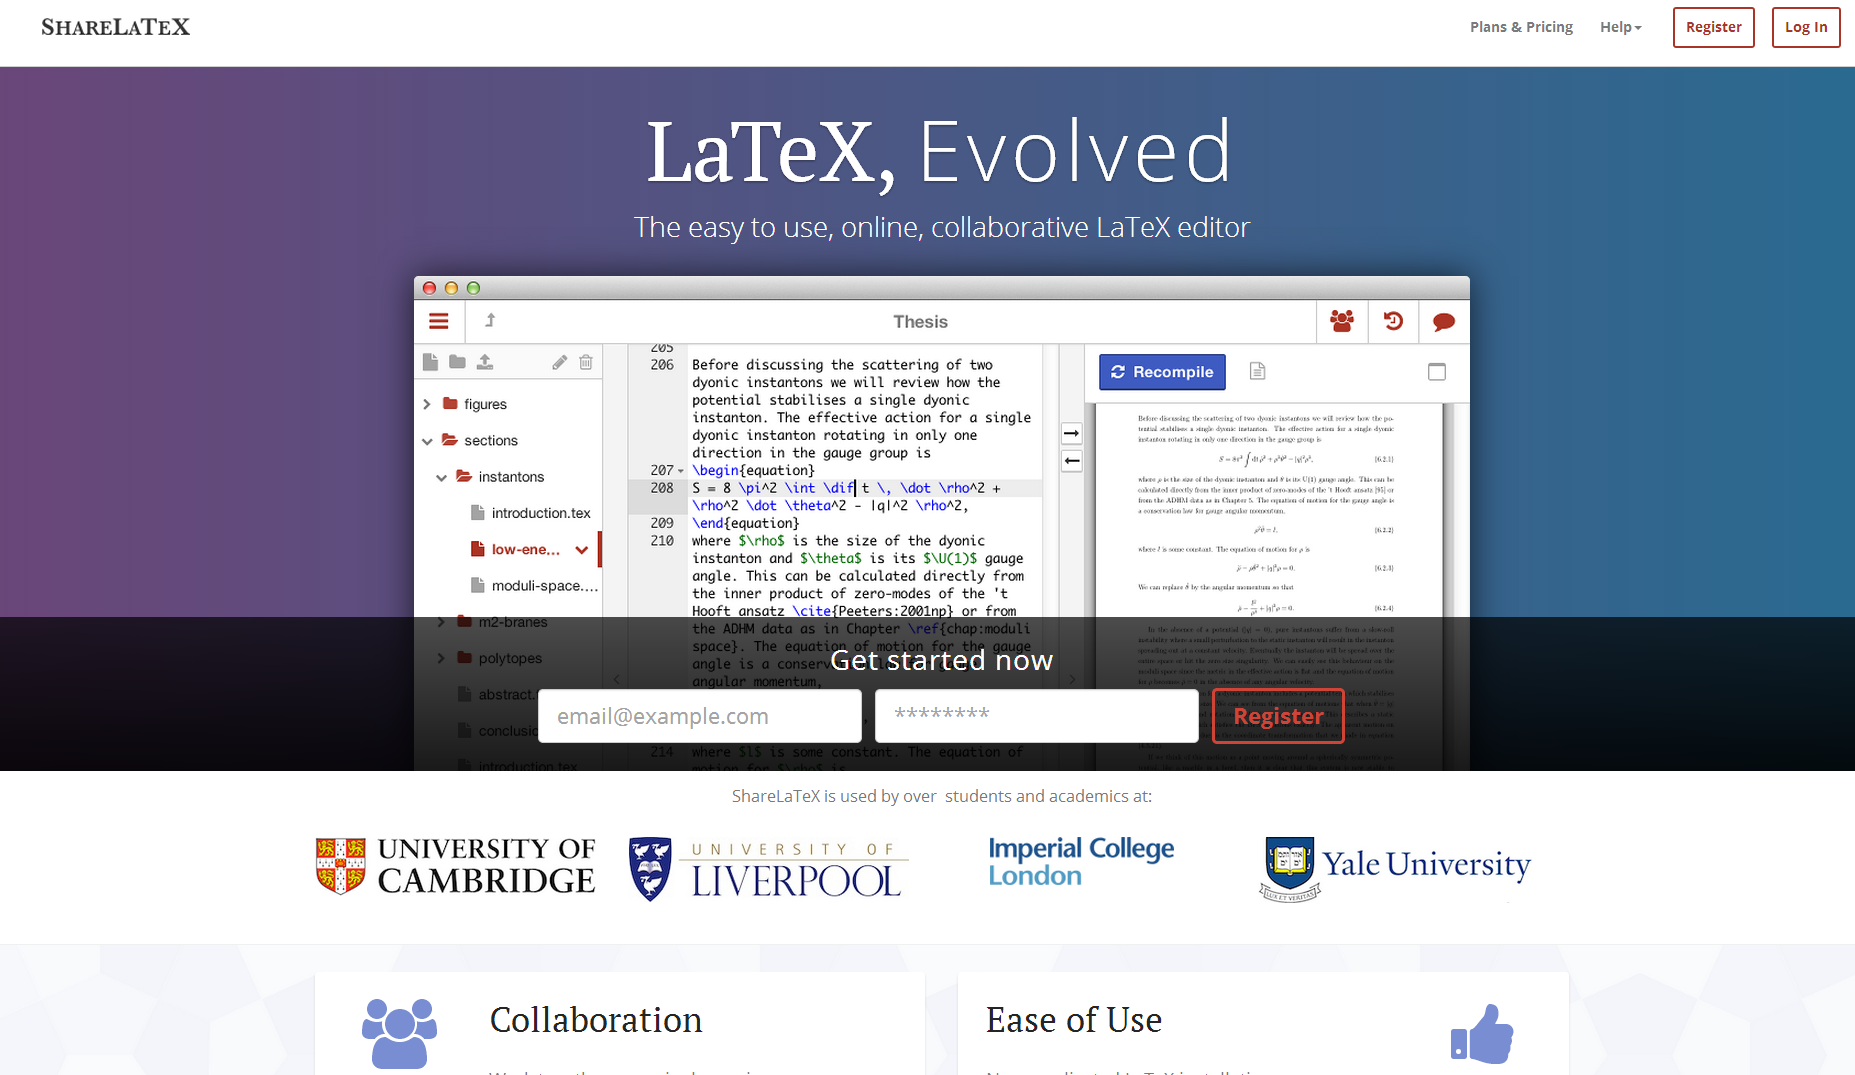
\includegraphics[width=0.65\linewidth]{images/ShareLaTeX_screenshot.png}}
\end{minipage}
\\[0.4cm]
\begin{minipage}[b]{\linewidth}
  \centering
  \url{https://www.writelatex.com}\\[4pt]
  \fbox{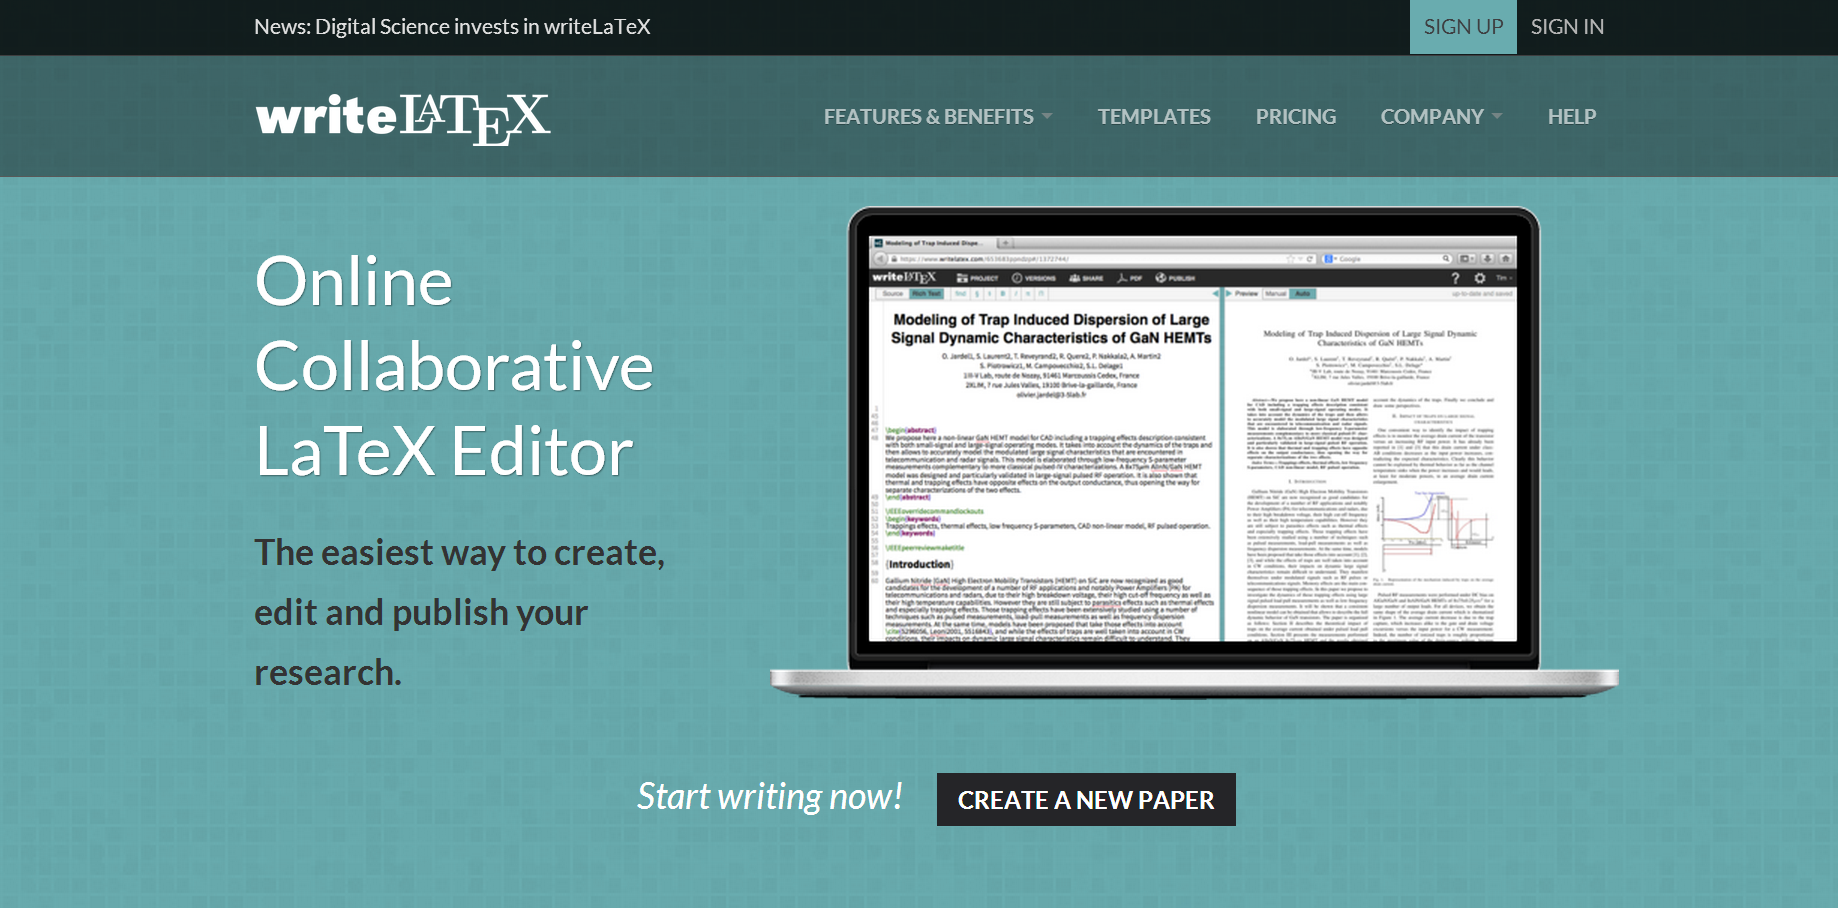
\includegraphics[width=0.65\linewidth]{images/writeLaTeX_screenshot.png}}
\end{minipage}
\\[0.4cm]
\begin{minipage}[b]{\linewidth}
  \centering
  \url{https://verbosus.com}\\[4pt]
  \fbox{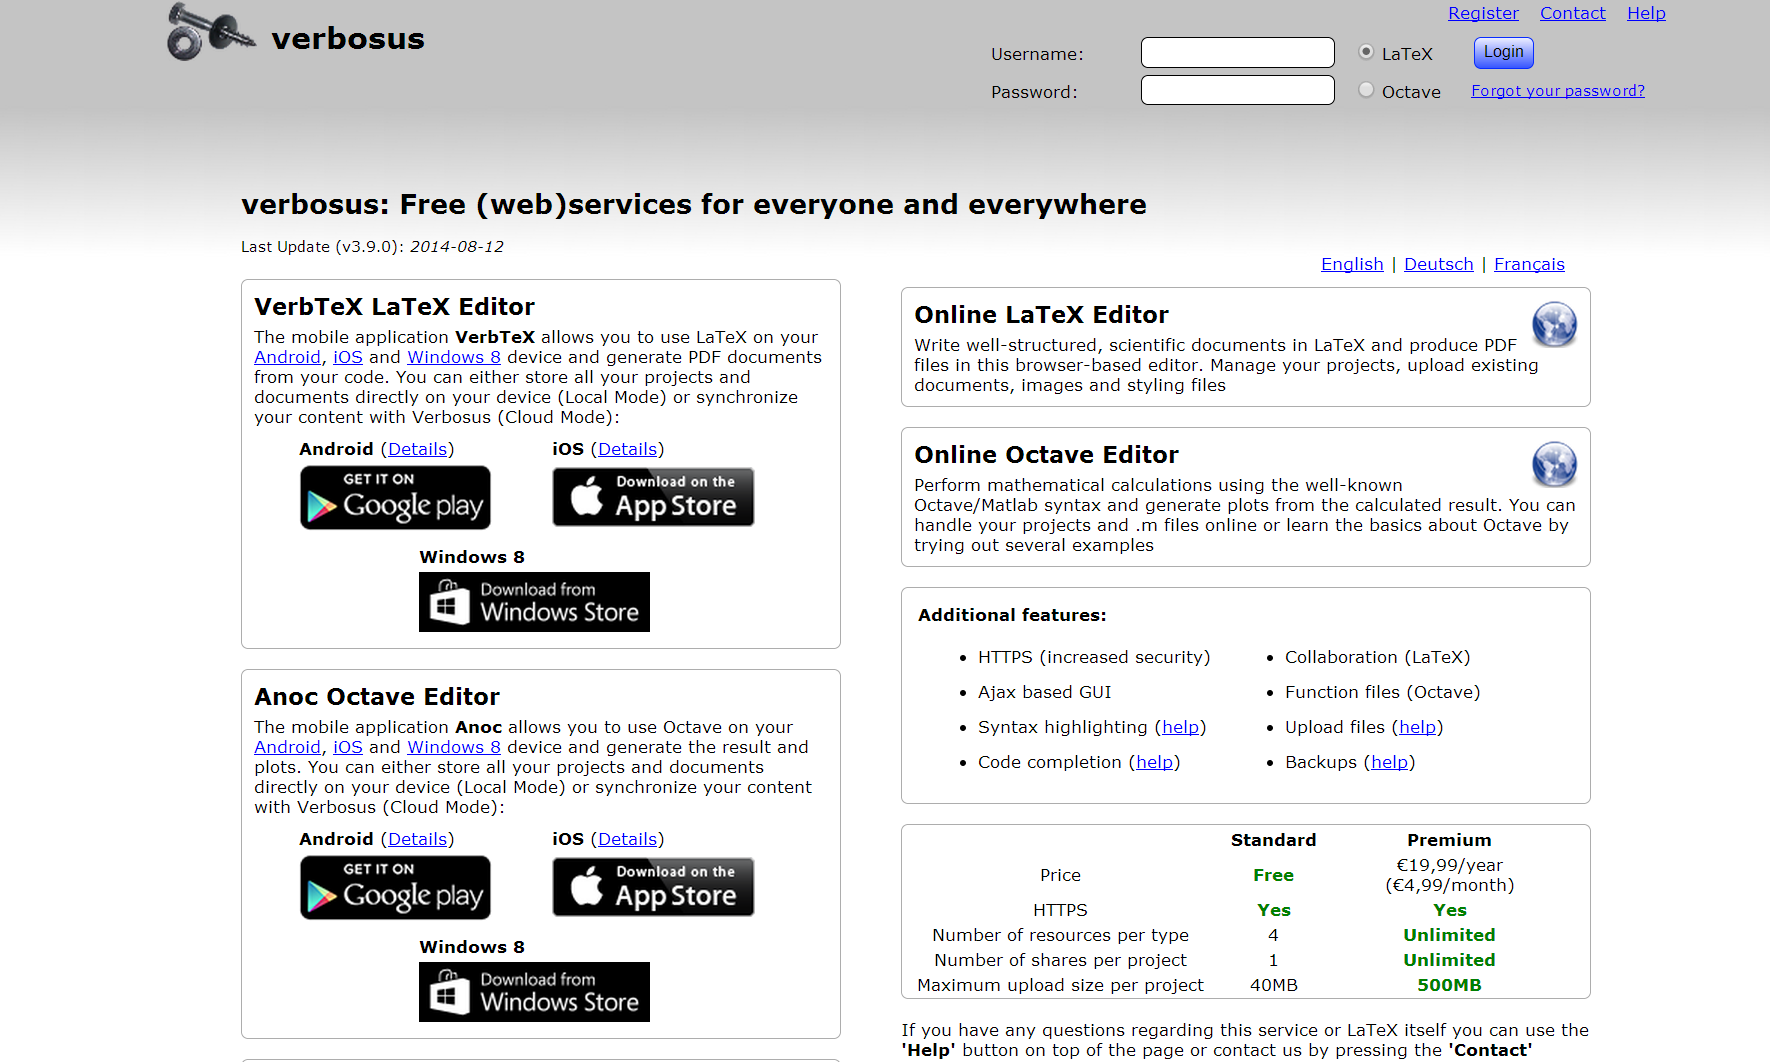
\includegraphics[width=0.65\linewidth]{images/verbosus_screenshot.png}}
\end{minipage}
\end{tabular}
\caption{Pagine di benvenuto di alcuni siti web 
  per la compilazione di documenti \LaTeX{} \emph{in the cloud}.}\label{fig:Online:Tools}
\end{figure*}

È utile visitare le sezioni di questi siti che offrono gratuitamente numerosi modelli di 
tesi di laurea.\footnote{\url{https://www.sharelatex.com/templates/thesis}}\footnote{\url{https://www.writelatex.com/templates}}

\backmatter
\bibliography{DeMarco_Tesi}

\printindex

\end{document}
